\documentclass{article}

\usepackage{amsmath}
\usepackage{fancyhdr}
\usepackage[square,sort,comma,numbers]{natbib}
\usepackage{amsfonts}
\usepackage[utf8]{inputenc}
\usepackage{graphicx}
\usepackage{multicol}
\usepackage{multirow}
\usepackage{subcaption}
\usepackage{hyperref}
\hypersetup{}
\urlstyle{same}

\pagestyle{fancy}
\fancyhf{}
\lhead{ \rightmark}
\rhead{ \thepage}
\renewcommand{\headrulewidth}{.5pt}

\usepackage{titlesec}
\titleformat*{\section}{\LARGE\bfseries}
\titleformat*{\subsection}{\Large\bfseries}
\titleformat*{\subsubsection}{\large\bfseries}
\titleformat{\paragraph}{\normalfont\normalsize\bfseries}{\theparagraph}{}{}
\titlespacing*{\paragraph}
{0pt}{3.25ex plus 1ex minus .2ex}{1.5ex plus .2ex}



\setlength{\parskip}{1em}
\graphicspath{ {./images/} }

\title{Sections and Chapters}
\author{Gubert Farnsworth}
\date{ }

\begin{document}
\maketitle
\tableofcontents

\newpage

% ==============================================================
% Introduction
% ==============================================================
\section{Introduction}

% ==============================================================
% GANS
% ==============================================================
\section{Background}
% ==============================================================

\pagebreak
% ==============================================================
\subsection{Generative Adversarial Networks}
% ==============================================================

Introduced in 2014 \cite{goodfellow_generative_2014}, generative adversarial  networks, so-called GANs, have been the focus of countless research papers and creative implementations. GANs have learned how to generate an image of a cat from a simple drawing \cite{hesse_image--image_nodate}, create new artworks \cite{rkjones4_gangogh_2018}, generate high-resolution celebrity faces \cite{karras_progressive_2017}, colorize grayscale images and much more.

In order to generate new realistic samples, two neural networks are trained to compete against each other. A common analogy can be found in money forgery: while a fraud investigator is trying to detect real bills from fraudulent ones, the money forger is trying to improve his falsification techniques, so that the investigator is unable to tell the difference.

In computational world, the investigator is a neural network called \textit{Discriminator} competing with the forger network called \textit{Generator}. The discriminator is trained to classify samples from the original dataset as ``real'', and samples generated by the generator as ``fake''. The generator is trained to fool the discriminator, so that it cannot correctly classify generated samples as fake.

Figure \ref{fig:mnist} shows example data points of the hand-written digits dataset MNIST \cite{lecun_mnist_nodate}, along with samples generated with a deep convolutional GAN \cite{kim_dcgan-tensorflow_2018} - the samples from the original and generated distributions are almost indistinguishable.

\begin{figure}[h]
\centering
\subcaptionbox{Original MNIST}
{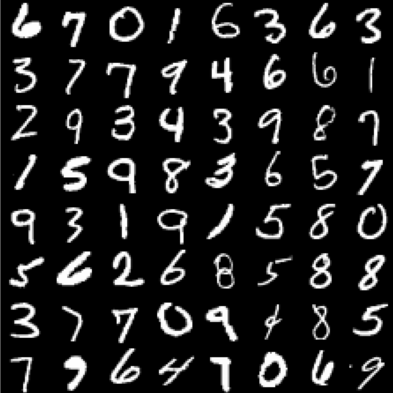
\includegraphics[height=4cm]{GAN/mnist_orig}}\hspace{1cm}
\subcaptionbox{Generated MNIST}
{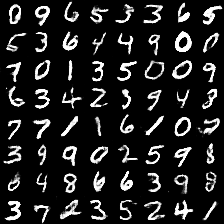
\includegraphics[height=4cm]{GAN/mnist_dcgan}}
\caption{\label{fig:mnist} \textbf{MNIST Example.}
(a) Example of data points in the original MNIST dataset \cite{lecun_mnist_nodate}. (b) Samples generated with a Deep Convolutional GAN \cite{kim_dcgan-tensorflow_2018}.}
\end{figure}



% ==============================================================
\subsubsection{Architecture}
% ==============================================================

Figure \ref{fig:gan} describes a typical GAN architecture. The discriminator is a common Convolutional Neural Network \cite{lecun_convolutional_1995}, which takes an image as input and is trained to extract necessary information in order to classify the image. The output is a scalar value, classifying the image as real or fake. 

The generator's architecture is similar, however it uses a transposed convolution, the so-called "deconvolution", to produce a 3-dimensional output from a 1-dimensional input vector. The generator input vector is sampled randomly.

The discriminator receives either a sample from the real data distribution, or a generated sample. The classification output of the discriminator is back-propagated  through the discriminator, as well as the generator network, in order to adjust the networks' weights to improve the training objective.

\begin{figure}[h]
\centering
{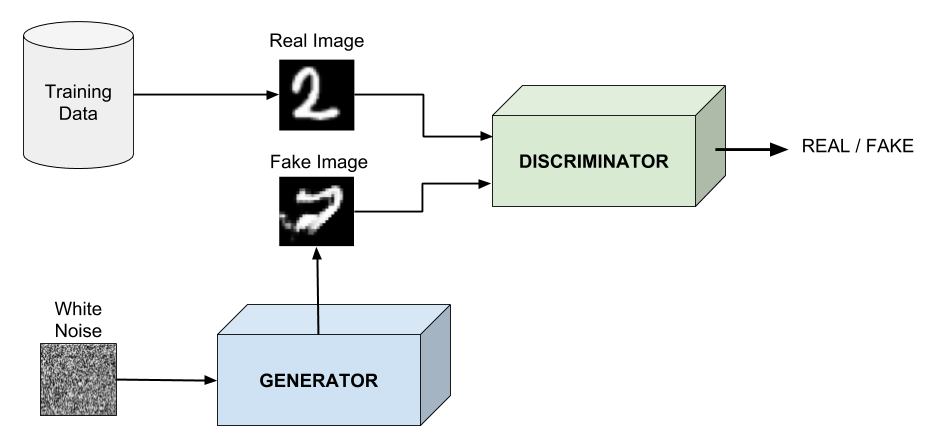
\includegraphics[width=\linewidth]{GAN/gan_model}}
\caption{\label{fig:gan} \textbf{GAN model.} The generator network produces fake images, which the discriminator network tries to distinguish from the real samples coming from the dataset.}
\end{figure}

% ==============================================================
\subsubsection{Training Objective} \label{sec:GAN_training}
% ==============================================================

Given input data with distribution $p(x)$, the generator $G$ is a neural network, that maps random input noise $z$ to the input space, as $G(z, \theta_{g})$, learning the model distribution $\hat{p}(x)$. The discriminator $D$ is a second neural network $D(x, \theta_{d})$ with a single scalar output, classifying the input $x$ as real, sampled from data distribution $p(x)$, or as fake, sampled from the model distribution $\hat{p}(x)$. 

The training objective of the discriminator is to maximize the probability of assigning the correct label, while the objective of the generator is to minimize this probability. The loss function of the GAN can be described as the minimax objective,

\begin{equation}
\underset{G}{\mathrm{min}} \ \underset{D}{\mathrm{max}} \ \mathcal{L}(D,G) = \mathbb{E}_{x \sim p_{data}(x)}[\log D(x)] + \mathbb{E}_{z \sim p_{z}(z)}[\log (1 - D(G(z))].
\label{eq:minimax}
\end{equation}

The gradient of this loss function is back-propagated through the networks in respect to each of the network's parameters, $\theta_{d}$ and $\theta_{g}$, followed by a parameter update using an optimization algorithm such as gradient descent.

% ==============================================================
\subsubsection{Training Difficulties} \label{sec:gan_diff}

In theory, the minimax game described in Equation \ref{eq:minimax} is played until generator has perfectly modeled the distribution $p(x)$, so that discriminator classifies the authenticity of the samples at random. In reality, the training of a GAN can prove to be unstable and finding the right balance between the two networks is difficult.

It can for example happen, that the gradient descent gets stuck in a cycle, where a modification to the discriminator weights reduces the discriminator loss and increases the generator loss, while the following modification of generator weights does the opposite \cite{salimans_improved_2016}. In this scenario, the gradient descent is not able to converge.

One of the common causes of instability is the vanishing gradient problem: when the discriminator gets confident at classifying the generated samples as fake early on, the generator gradient vanishes and the generator has no chance to improve. 

In the original GAN paper, Goodfellow et al. \cite{goodfellow_generative_2014} suggest $G$ to be trained to maximize $\mathbb{E}_{z \sim p_{z}(z)}[\log D(G(z))]$, instead of the original term used in Equation \ref{eq:minimax}, to avoid vanishing gradients. 

Since then, other research on how to stabilize GAN training has been published \cite{arjovsky_towards_2017}\cite{roth_stabilizing_2017}\cite{salimans_improved_2016}. The recommended techniques to prevent the vanishing gradient problem mostly try to to confuse the discriminator, to give the generator an advantage in the training. 

One of the techniques that can be applied is to add noise to the labels that define if the image is real (1.0) or fake (0.0). As shown by Saliman et al. \cite{salimans_improved_2016}, varying the labels with a slight noise can help to stabilize the training. To further confuse the discriminator, we can also occassionally flip the labels. 

% ==============================================================
% Deep Convolutional GANs
% ==============================================================
\subsubsection{Deep Convolutional GANs} \label{sec:dcgan}


Many GAN implementations base their network architecture on Deep Convolutional GANs, described by \cite{radford_unsupervised_2015}. The authors introduced architectural guidelines for convolutional networks used in GANs, that stabilize the training and result in more realistic outputs.

\begin{figure}[h]
\centering
{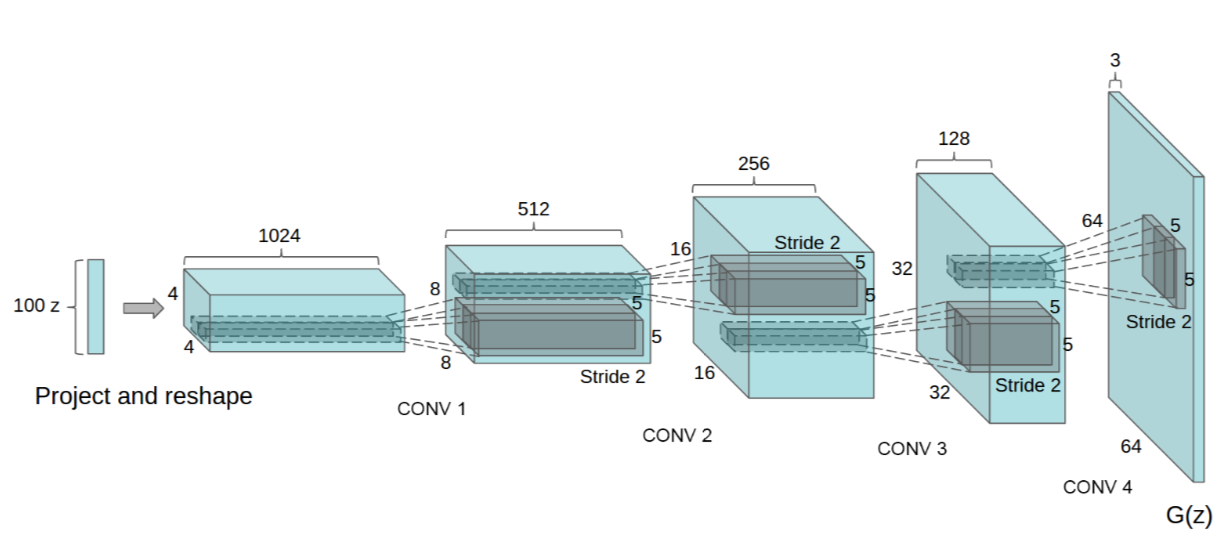
\includegraphics[width=\linewidth]{GAN/dcgan_generator}}
\caption{\label{fig:dcgan} \textbf{DCGAN Generator.} An example architecture of a DCGAN generator $G(z)$. The random input noise $z$ is mapped to a 64x64 image with 3 color channels via fractionally-strided convolution layers. Figure reprinted from \cite{radford_unsupervised_2015}.}
\end{figure}


After experimenting with CNN architectures commonly used in computer vision tasks, Radford et al. \cite{radford_unsupervised_2015} have found that this set of architecture modifications has a positive effect on the stability and convergence speed of the models:
\begin{itemize}
\item \textbf{All Convolutional Net}: A common practice in convolutional neural networks are \textit{Pooling Layers}, which reduce the number of parameters by filtering the convolution outputs, taking maximum or average of a given region. However, the authors have found that using an All Convolutional Network \cite{springenberg_striving_2014}, which replaces all pooling layers with a strided convolution, leads to more stable results.
\item \textbf{Fully-Connected Layers}: The authors argue, that avoiding fully-connected layers deeper in the network stabilizes the network. They keep fully-connected layers only in the discriminator output layer and generator input layer, as removing these would slow down the convergence.
\item \textbf{Batch Normalization}: Batch Normalization \cite{ioffe_batch_2015} has been introduced in common image-classification to make models more robust to parameter initialization and speed up training. The DCGAN paper shows that including a batch-norm layer in all GAN layers (except discriminator output and generator input), helps generators start learning and produce diverse outputs.
\item \textbf{Activation Functions}: As opposed to maxout activation suggested by the original GAN paper \cite{goodfellow_generative_2014}, GANs seem to benefit from \textit{Leaky ReLU} activation function in discriminator, and \textit{ReLU} activation function for generator, except last generator layer, which uses a \textit{tanh} activation function.
\end{itemize}

The DCGAN architecture established itself as the state-of-the-art architecture and is the model for most of the GAN implementations mentioned in this thesis.

% ==============================================================
% Conditional GANs
% ==============================================================
\subsubsection{Conditional GANs} \label{sec:cond_gan}
Mirza and Osindero \cite{mirza_conditional_2014} introduced the Conditional Generative Adversarial Networks to be able to influence the output of a GAN. By conditioning both the discriminator and the generator on additional information, the generator learns to output realistic samples based on given input.

Considering the previous example of MNIST hand-written digits synthesis, one can condition the networks using the digits as class labels, and control the network to generate an image of a specific digit. There have also been experiments with text-to-image translation \cite{reed_generative_2016}, where the network is conditioned on a text description of an image, and various image-to-image translation GANs \cite{yoo_pixel-level_2016}\cite{yoo_pixel-level_2016}\cite{pathak_context_2016}.

The training objective of conditional GAN is following:
\begin{equation}
\underset{G}{\mathrm{min}} \ \underset{D}{\mathrm{max}} \ V(D,G) = \mathbb{E}_{x \sim p_{data}(x)}[\log D(x|c)] + \mathbb{E}_{z \sim p_{z}(z)}[\log 1 - D(G(z|c))].
\label{eq:cgan}
\end{equation}

The conditioning information $c$, such as a class label, text, or another image, is fed to both discriminator $D$ and generator $G$ as additional input layers.









\pagebreak
% ==============================================================
% Image Retrieval
% ==============================================================
\subsection{Content-Based Image Retrieval}
The idea of content-based image retrieval systems, also called CBIR, is to find semantically similar images without depending on textual meta-data, such as tags or descriptions. Instead these systems only rely on the pixel values and try to find similarities based on visual features that can be extracted from the content of the images.

CBIR is a field of computer vision that has seen a lot of changes since the rise of fast and available deep learning algorithms. While the first CBIR implementations have relied on low-level features such as color and texture to identify similar images, today the state-of-art techniques rely on high-dimensional descriptors produced by convolutional neural networks.

The systems are used for many specific applications in different fields, e.g: medicine, retail or archives. Many CBIR systems are also freely available online, such as the visual image search on Google, or a tool for exploring large amounts of images based on their similarities \cite{Barthel:2017:VBM:3078971.3079016}.


\begin{figure}[h]
\centering
{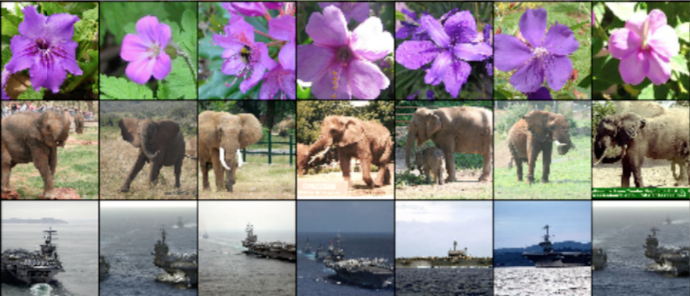
\includegraphics[width=\linewidth]{CBIR/cnn_cbir}}
\caption{\label{fig:conv_cbir} \textbf{Image Retrieval with CNN Features}. The test image on the left is compared to images from the train set to find most similar matches. The images are compared based on 4028-dimensional feature vectors extracted from the last hidden layer of a convolutional neural network. Figure reprinted from \cite{NIPS2012_4824}.}
\end{figure}


\pagebreak
\subsubsection{Low-Level Visual Features}

\paragraph{Color Features}
Color is one of the most basic features of an image. While there are many possibilities to describe the color of an image, such as average color or selecting a few dominant colors, the color histogram has proven to be a robust choice and is often used as a baseline when comparing other color features \cite{Torres_content-basedimage}.

To create a color histogram, the number each color (described by the image's discrete color space, such as RGB) occurs in the image is counted. The counts can be grouped into various amount of bins and represented as relative frequencies \cite{Swain1991}.

\begin{figure}[h]
\centering
\subcaptionbox{RGB Image}{\includegraphics[height=5cm]{CBIR/atacama}}
\subcaptionbox{3D Color Histogram}{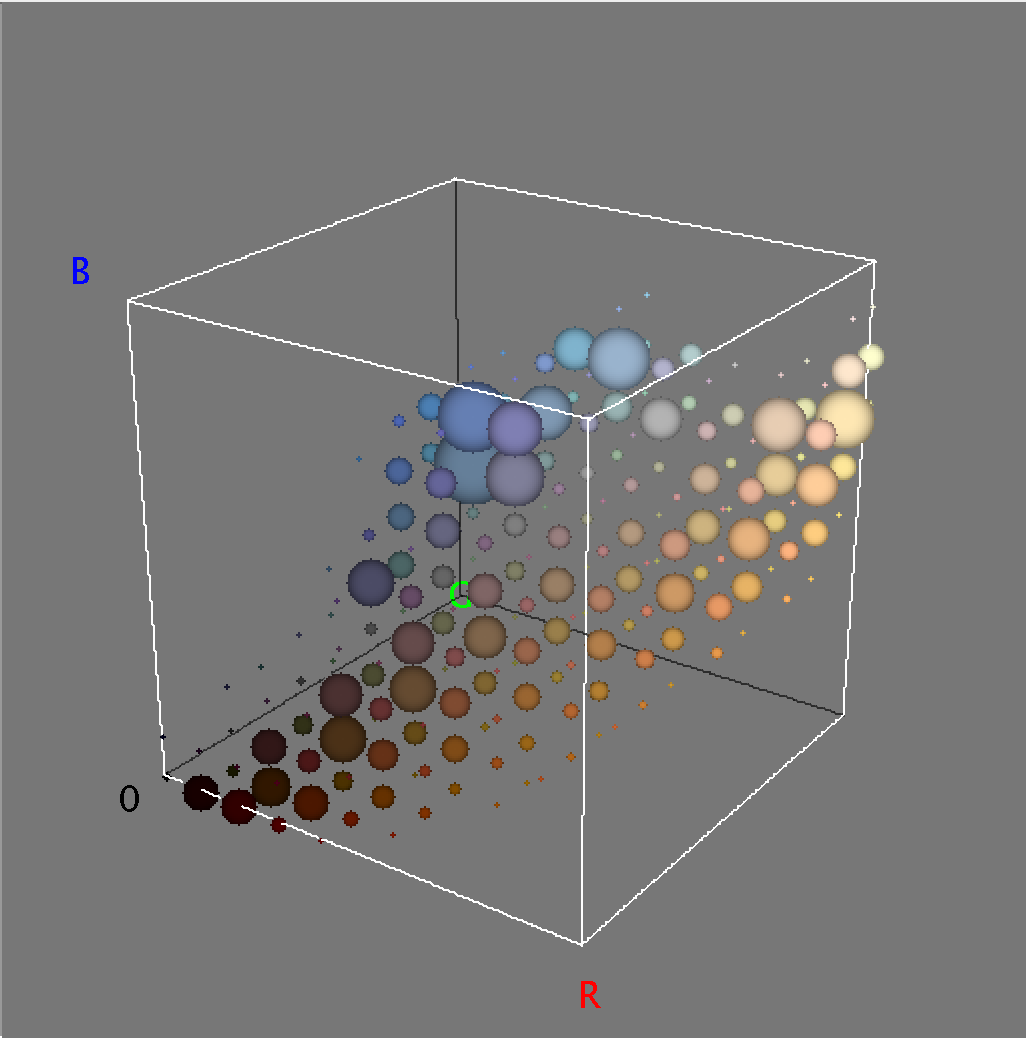
\includegraphics[height=5cm]{CBIR/color_hist}}
\caption{\label{fig:color_hist} \textbf{Color Histogram}. A 3-D visualization of the color histogram with 200 color bins for an RGB image. Histogram visualization created with 3D Color Inspector \cite{barthel_3d_nodate}.}
\end{figure}

The main advantage of color features is that they are invariant to image transformations such as rotation. However, basing the retrieval only on colors is insufficient, since images that share similar color histograms do not necessarily display the same content and images showing the same content can have different color palettes.


\paragraph{Shape Features}
Shape features can be divided into two groups: \textit{contour-based} features which only extract the edges of the shape, or \textit{region-based} features which extract the edges together with their interior \cite{zhang2004review}. Figure \ref{fig:shape_feat} shows the difference between these two groups.

Various methods for shape extraction have been developed, however, most of them have difficulties dealing with the projection of real world 3-D object onto a 2-D image and can also struggle with abnormalities created by lighting and shadows \cite{zhang2004review}.

\begin{figure}[h]
\centering
{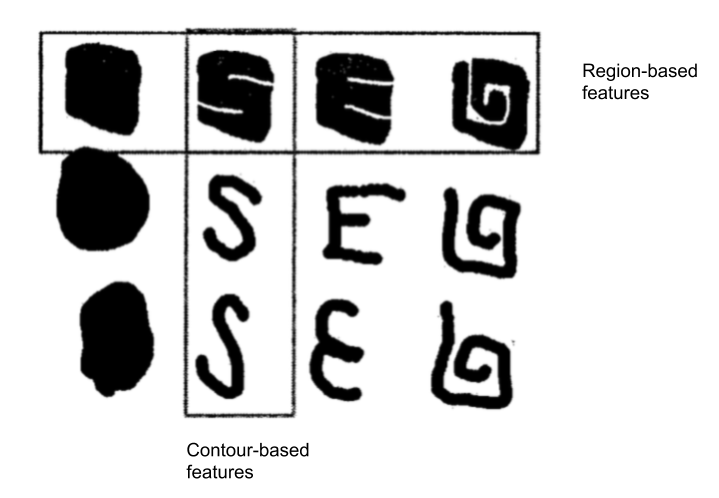
\includegraphics[height=5cm]{CBIR/shape_features}}
\caption{\label{fig:shape_feat} \textbf{Shape Features}. The highlighted row shows images considered similar based on region shape feature, and the highlighted column shows contour-based similarity. Figure reprinted from \cite{bober_mpeg-7_2001}}.
\end{figure}

\paragraph{Texture Features}
Although texture can be perceived equally important to color, it is more difficult to define it.  Some of the terms to describe texture, as defined by Tamura et al \cite{tamura1978textural}, are contrast, directionality, line-likeness, and regularity.

There are several methods for extracting texture that can be based on statistics, such as the co-occurence matrix, human perception, such as Tamura features, or signal processing, such as Gabor filters or Fourier transformations.

\paragraph{MPEG-7}
The MPEG-7 standards were developed to describe the contents of images, audio and video independently from their format. They provide various low-level feature descriptors of color, shape, texture, motion and others, that enable fast and efficient multimedia search \cite{noauthor_visual_nodate}.

Many of these descriptors are widely used in CBIR systems, such as the color layout, edge histogram or 3D shape descriptor.

\pagebreak
\subsubsection{CNN Features}
Convolutional Neural Networks, also known as ConvNets or CNNs, are the state-of-the-art neural networks for most computer vision tasks, such as image classification and object detection or face recognition. Various research has also shown that a ConvNet can produce very powerful image descriptors, which can be used for image retrieval \cite{razavian_cnn_2014-2}, \cite{NIPS2012_4824}.

Unlike regular feed-forward neural networks based on fully-connected layers of neurons, ConvNets are trained to learn relatively small filter kernels, that can extract valuable information from different areas of an image. Therefore, they reduce the amount of training parameters significantly and are able to train also on large images.

As shown in Figure \ref{fig:conv_feats}, in the early layers of the network, the filters learn to recognize simple visual features, such as horizontal edges or colors. The filters recognize more complex structures as the network's layers get deeper. In the last layers of the network, the filters are trained to recognize high-level features. 

\begin{figure}[h]
\centering
\subcaptionbox{Low-Level Features}{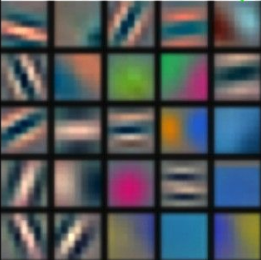
\includegraphics[height=3.5cm]{CBIR/feat_low}}\hspace{.3cm}
\subcaptionbox{Mid-Level Features}{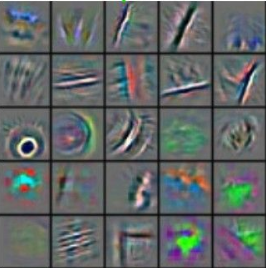
\includegraphics[height=3.5cm]{CBIR/feat_mid}}\hspace{.3cm}
\subcaptionbox{High-Level Features}{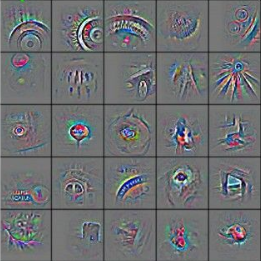
\includegraphics[height=3.5cm]{CBIR/feat_high}}
\caption{\label{fig:conv_feats} \textbf{Convolutional Feature Maps}. Each image displays a sample of feature maps (filters) from different layers of the networks. The early layer feature maps recognize simple patterns, while the last layers recognize more complex structures. Figure adapted from \cite{gandhi_build_2018}.}
\end{figure}


Krizhevsky et al. \cite{NIPS2012_4824} use a ConvNet, trained to classify more than 1 million images into 1000 classes, to extract 4028-dimensional image features from the last hidden layer of the network. They show, that these feature vectors can be used to find images with similar content and are invariant to the position of the objects in the image, lighting and colors. Their results are shown in Figure \ref{fig:conv_cbir}.


\pagebreak
\subsubsection{Distance Metrics}
To retrieve relevant images, distances between the extracted image features need to be evaluated based on a metric. The most commonly used metrics is the \textit{L1 norm}, also called \textit{Manhattan distance}, and \textit{L2 norm}, also known as \textit{Euclidean distance}.

Given two $n$-dimensional vectors vector $x = (x_1, x_2, ..., x_n)$ and $y = (y_1, y_2, ..., y_n)$, the L1 distance is computed by summing up the absolute values of the difference between the respective coordinates of the vectors:
\begin{equation}
L_1(x, y) = \sum_{i=1}^{n} |x_i - y_i|.
\end{equation} 

L2 distance is the squared root of sum of squared distances between respective vector coordinates:
\begin{equation}
L_2(x, y) = \sqrt{\sum_{i=1}^{n} (x_i - y_i)^2}.
\end{equation}

There are also other possible metrics like the \textit{Chebychev metric} or the \textit{Minkowski Metric}.


\pagebreak
% ==============================================================
\section{Analysis}
% ==============================================================

% ==============================================================
% DATA
% ==============================================================
\subsection{Data} \label{sec:data}
As in most machine learning algorithms applied to visual tasks, the quantity and quality of training data is essential to produce high-quality results. It is also common, that data collection and data cleaning make up a significant part of a machine learning project.

In case of fashion images, there are several open-source datasets published online. However, after careful evaluation I have not found them sufficient for the purpose of this thesis. Therefore I have created an application to scrape online fashion stores and download images of fashion products and their description in a computer-readable format.

% ==============================================================
\subsubsection{Requirements}
% ==============================================================

In order to generate high-quality outputs using GANs, the collected dataset should fulfill the following requirements:
\begin{enumerate}
\item The fashion products should be photographed on a white background. 
\item There should be a machine-readable description of each product, such as color, shape, category, etc. 
\item The images should be in a sufficient resolution.
\item There should be a sufficient amount of images of various items.

\end{enumerate}
I have defined these requirements based on my previous experience with generative algorithms. It is generally easier for the algorithm to focus on the important attributes of the images, if there are no distractions in terms of different model poses, backgrounds, etc. And since the main point of the project is to modify different attributes of the products, the images need to be labeled.

\pagebreak
\subsubsection{Existing Fashion Datasets}
\paragraph{DeepFashion}
The Deep Fashion Set \cite{liu2016deepfashion} includes more than 200.000 images of clothing images, labeled with 1.000 attributes. However, this dataset does not fulfill the first requirement of the dataset - its clothing items are photographed on people in various poses and backgrounds. This type of variation might be too complex for the algorithms and can lead to unsatisfactory results.

\paragraph{Fotolia}
Another available option, that has been provided by Prof. Dr. Barthel, is the Fotolia image dataset, which can be explored on the picsbuffet website \cite{noauthor_picsbuffet_nodate}. 

To test the dataset, I have chosen all images with keywords ``dress'' and ``isolated'' and compared them to a template image, based on the distance between their 64-dimensional feature vectors calculated via Akiwi API \cite{sonnenberg_akiwi_nodate}. Figure \ref{fig:fotolia} shows the results of this search. 

Additionally to an undesired low resolution of the returned images - around 100 x 160 pixels - the results also have too much variety, such as different model poses, different zoom levels and backgrounds. The description of the images did not include many useful attributes, with most pictures being labeled with words such as: ``beauty'', ``young'', ``person'', and lacking information about colors, shapes and pattern.

\begin{figure}[h]
\centering
\subcaptionbox{Template Image}{\fbox{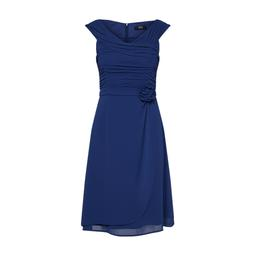
\includegraphics[height=3cm]{dress_template}}}\hspace{1cm}
\subcaptionbox{Fotolia Images}{\fbox{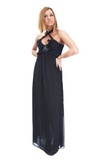
\includegraphics[height=3cm]{fotolia_ex1}}
\fbox{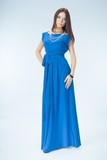
\includegraphics[height=3cm]{fotolia_ex2}}
\fbox{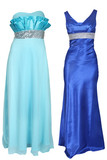
\includegraphics[height=3cm]{fotolia_ex3}}}
\caption{\label{fig:fotolia} \textbf{Fotolia images} The retrieved Fotolia images (b) with keywords ``dress'' and ``isolated'' with smallest feature vector distance from the template image (a).}
\end{figure}

\pagebreak
% ==============================================================
\subsubsection{Scraped Dataset}
% ==============================================================
Based on the evaluation of existing fashion datasets, I have identified a need for creating a new dataset specifically for the requirements of the application. I evaluated several fashion e-shops, from which images of the products and their descriptions could be downloaded. 

I chose 3 websites, based on the structure and amount of information they provide: \href{https://www.zalando.de/damen-home/}{zalando.de}, \href{https://www.aboutyou.de/}{aboutyou.de} and \href{https://www.fashionid.de/damen/}{fashionid.de}. Each of them provides several thousand fashion products for women and men, with a photograph of the item on a white background and some basic description such as color, pattern, shape, length etc. For simplicity, I have limited the dataset to women's clothes, excluding products like accessories and shoes.

The \textit{Fashion Scraper} is a python project, that scrapes images and data from all the mentioned websites and saves them locally for further processing, such as image processing, data cleaning, and description translating. This project was part of my Independent Coursework and the documentation of the project can be found in Attachments, or on \href{https://github.com/sonynka/fashion_scraper}{github.com/sonynka/fashion\_scraper}.

\begin{figure}[h]
\centering
{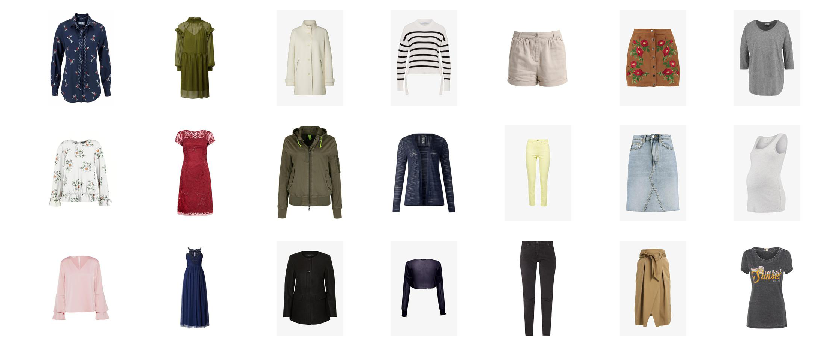
\includegraphics[width=\linewidth]{dataset_examples/img_grid2}}
\caption{\label{fig:dataset} \textbf{Examples of images in the final dataset.} Each column contains images from different category as follows: blouses, dresses, jackets, knitwear, pants, skirts, tops.}
\end{figure}

The scraped dataset consists of 92.200 images of size $256\times256$ pixels in JPEG format. The images are split into folders by categories and the whole dataset is described in a CSV file, which includes the following information:
\pagebreak
\begin{itemize}
\item \textbf{id}: ID of the product as defined by the website (SKU)
\item \textbf{img\_path}: relative local file path to the saved product image
\item \textbf{img\_url}: URL to the product image file hosted on the seller website
\item \textbf{model\_img\_urls}: URLs to the images of the product worn by models
\item \textbf{product\_url}: if given, the URL to the product listing on the website
\item \textbf{brand}: product brand as displayed on the website
\item \textbf{name}: product name as displayed on the website
\item \textbf{attributes}: list of product attributes listed on the website in German, such as shape, length, material, size etc.
\end{itemize}

In addition to the website data, there are columns that contain processed and translated data. Below is the list of the column names and the values they can take.
\begin{itemize}
\item \textbf{category}: blouses, dresses, jackets, knitwear, pants, skirts, tops
\item \textbf{color}: beige, black, blue, gray, green, pink, red, white, yellow
\item \textbf{length}: 3-4, knee, long, normal, short or no value
\item \textbf{sleeve\_length}: half, long, short, sleeveless or no value
\item \textbf{fit}: loose, normal, tight or no value
\item \textbf{pattern}: floral, lace, polkadots, print, stripes, unicolors or no value
\item \textbf{neckline}: back, deep, lines, round, v, wide or no value
\end{itemize}

\marginpar{A table with all attributes and num of images will be in attachments}
There is also a CSV file that contains a list of image file paths and binary classification of the list of values mentioned in the above list.

\pagebreak
\paragraph{Model Images}
For some experiments I also downloaded an extra dataset of images of products worn by models from the scraped websites. The model images are of size $256\times256$ pixels in JPEG format and the file names correspond to the file names of the product images. Each product has variable amount of corresponding model images, varying in model poses, zoom level and detail level of the photo (see Figure \ref{fig:models}).

\begin{figure}[h]
\centering
{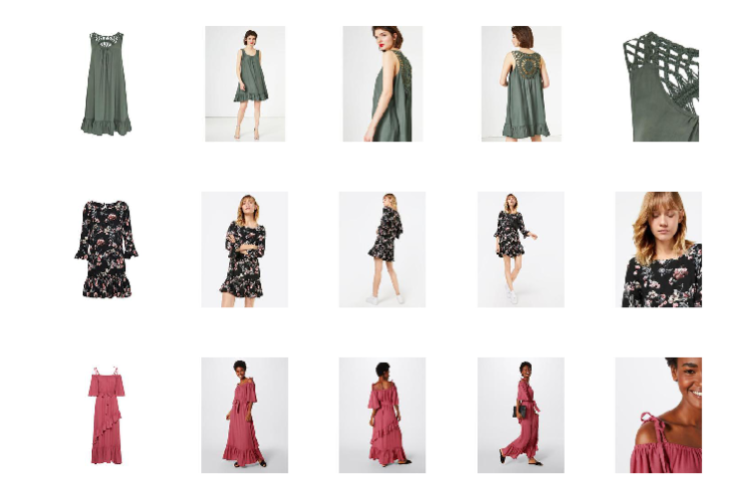
\includegraphics[width=\linewidth]{dataset_examples/model_images}}
\caption{\label{fig:models} \textbf{Examples of model images in the dataset.} First column shows the product images and the other columns show images of models wearing the given product in various poses and level of detail.}
\end{figure}

\pagebreak
% ==============================================================
\subsection{Image-To-Image Translation}
% ==============================================================
Image-To-Image Translation using GANs has been widely researched in the past few years, with creative approaches and models published regularly. For the purpose of this thesis, I have reviewed and tested some of these projects, to evaluate what results can be achieved on the fashion dataset and which GAN is best suited for what task.

Table \ref{tab:gan_comp} shows the comparison of 5 evaluated networks: \textit{pix2pix} \cite{isola_image--image_2016}, \textit{CycleGAN} \cite{zhu_unpaired_2017}, \textit{StarGAN} \cite{choi_stargan_2017}, \textit{MUNIT} \cite{huang_multimodal_2018} and \textit{FaderNetworks} \cite{lample_fader_2017}, for which I compared the following attributes:
\begin{itemize}
\item \textbf{Supervised}: Does the network need a dataset consisting of paired images, such as the same skirt in a short and long version.
\item \textbf{Multi-Domain}: Is the network able to train one model for different domains translations, or does each domain pair require its own trained generator.
\item \textbf{Multi-Modal}: Is the network able to generate different outputs from the same input.
\item \textbf{Latent representations}: Does the network train in pixel-space or uses latent representations, such as separate content and style representations.
\end{itemize}

The following sections describe the characteristics of the evaluated networks, their applications, training process and architecture.

\begin{table}[h]
\centering
\begin{tabular}{l*{5}{c}}
Characteristics & pix2pix &	CycleGAN & StarGAN	& MUNIT	& FaderNets \\
\hline
Supervised				& Yes & No & No & No & No \\
Multi-Domain  			& No  & No & Yes & No & No \\
Multi-Modal				& No & No & No & Yes & No \\
Latent Space 			& No & No & No & Yes & Yes \\
\end{tabular}
\caption{\label{tab:gan_comp}\textbf{Comparison of existing GAN models based on their characteristics.} %Supervised training means that the dataset consists of image pairs, e.g: a dress and a person wearing the dress. Multi-Domain networks are able to train one model to change multiple attributes. Multi-Modal networks are able to generate more than one possible output. Networks with latent representations try to model the training data in a latent space, as opposed to pixel space.
}
\end{table}

\pagebreak
\subsubsection{Pix2Pix}
The so-called Pi2Pix networks were first introduced by Isola et al. \cite{isola_image--image_2016} as a framework for image-to-image translations. Some of the applications of Pix2Pix include mapping day photographs to night, sketches of shoes to realistic shoe images or colorizing black-and-white photos (Figure \ref{fig:pix2pix_example}).

\begin{figure}[h]
\centering
{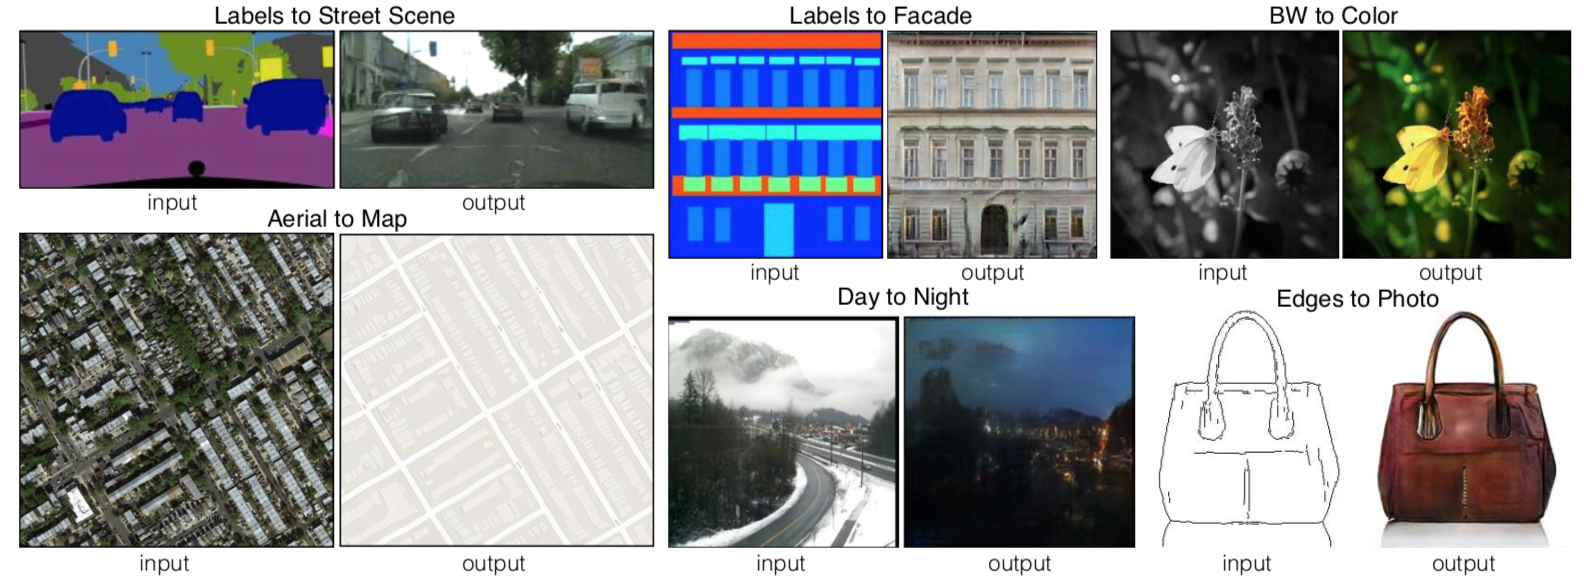
\includegraphics[width=\linewidth]{GAN/pix2pix_example}}
\caption{\label{fig:pix2pix_example} \textbf{Pix2Pix: Examples of translation between various domains.} Use cases of the pix2pix framework include translating day images to night or colorizing grayscale images. Figure reprinted from \cite{hesse_image--image_nodate-1}.}
\end{figure}

Pix2Pix uses the concept of conditional GANs \cite{mirza_conditional_2014} (described in Section \ref{sec:cond_gan}) to influence the network's output by providing a condition. In case of Pix2Pix, the condition is an image that is to be translated to another domain. To translate images from an input domain to a target domain, the model requires a dataset of paired images $(x_{input}, x_{target})$, such as a grayscale image and a corresponding color image. 


\begin{figure}[h]
\centering
{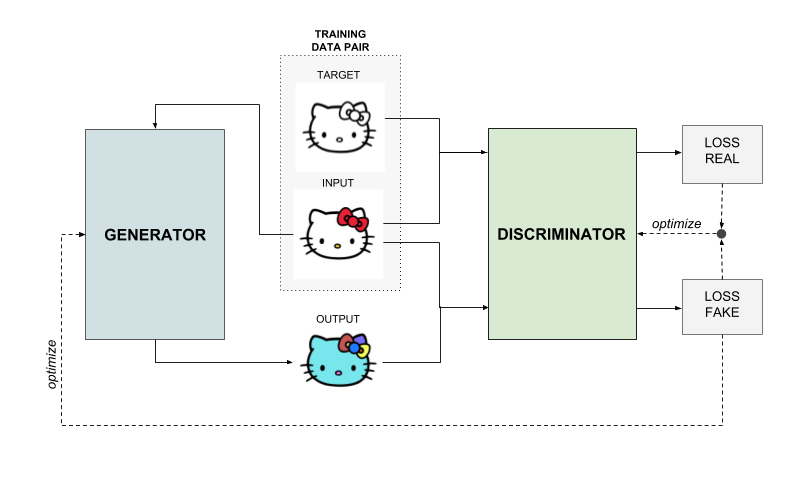
\includegraphics[width=\linewidth]{GAN/pix2pix}}
\caption{\label{fig:pix2pix} \textbf{Pix2Pix Training Process.} Dataset consists of paired input and target images. Generator takes input image as condition to output a generated image. Discriminator tries to predict, given the input image, if the target image comes from dataset or from generator. This output is then used to further optimize both networks. Figure adapted from \cite{hesse_image--image_nodate-1}.}
\end{figure}

As shown in Figure \ref{fig:pix2pix}, the generator takes the input image $x_{input}$ and tries to map it to the target domain $\hat{x}_{target}$, such as: $G: (x_{input}, z) \rightarrow \hat{x}_{target}$. The discriminator, also conditioned on the input image $x_{input}$, tries to predict if the target image comes from the data distribution or if it was generated. The discriminator tries to improve these classifications, while the generator tries to prevent correct classification.


\paragraph{Training Objective}
The adversarial objective, which $G$ is trained to minimize and $D$ is trained to maximize, can be expressed as following:
\begin{equation}
\underset{G}{\mathrm{min}} \ \underset{D}{\mathrm{max}} \ \mathcal{L}_{adv}(D,G) = \mathbb{E}_{x_{in},x_{trg}}[\log D(x_{in},x_{trg})] + \mathbb{E}_{x_{in},z}[\log 1 - D(x_{in}, G(x_{in},z))]
\label{eq:pix2pix_minimax_cond}
\end{equation}

Based on the results of previous conditional GAN approaches \cite{pathak_context_2016}, Isola et. al \cite{isola_image--image_2016} have also shown, that enforcing the generated output to be closer to the ground truth target by adding a second objective reduces artifacts in the results. They therefore suggest to use the L1 distance as reconstruction loss function for the generator to optimize.
\begin{equation}
\mathcal{L}_{rec}(G) = \mathbb{E}_{x_{in},x_{trg},z}[||x_{trg}-G(x_{in},z)||_{1}]
\label{eq:pix2pix_loss_rec}
\end{equation}

The final objective of the generator is:
\begin{equation}
\mathcal{L} = arg \ \underset{G}{\mathrm{min}} \ \underset{D}{\mathrm{max}} \ \mathcal{L}_{adv}(D,G) + \lambda \mathcal{L}_{rec}(G)
\end{equation}
where $\lambda$ controls the relative importance of the two loss functions.


\paragraph{Generator}
In image translation tasks, it is usual, and even desirable, that the input and target image domains share a common underlying structure. Modeling the generator with a simple encoder-decoder architecture, where all data must pass through a so-called "bottleneck" layer, can therefore result in an undesirable loss of the low-level details that the two domains share. 

The authors therefore suggest to base the generator on a U-Net architecture. U-Net contains so-called skip connections, which pass the output directly from the encoder to the decoder, therefore skipping the bottleneck. The generator is therefore able to include low-level features from the input in the output.

\begin{figure}[h]
\centering
{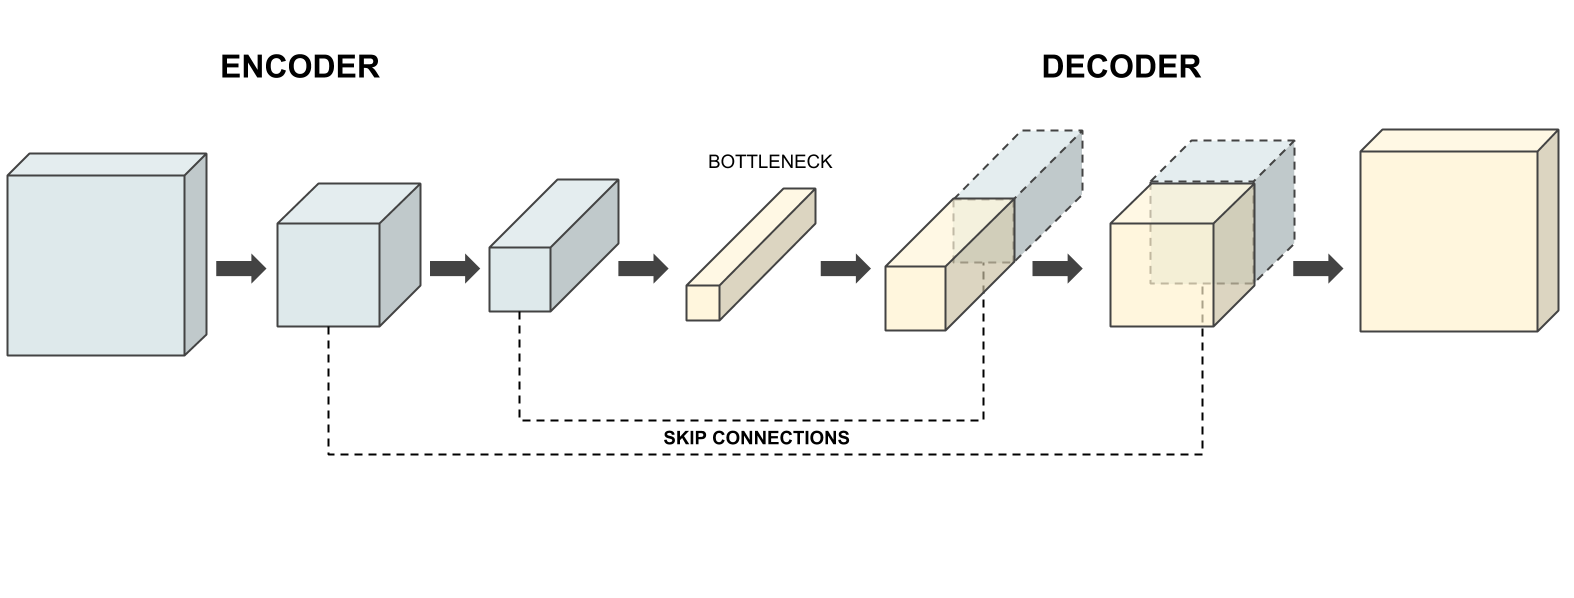
\includegraphics[width=\linewidth]{GAN/u-net}}
\caption{\label{fig:u-net} \textbf{U-Net Generator.} Skip connections are added between each encoder layer $i$ and decoder layer $n - i$, where $n$ is the total number of layers, so that information can bypass the bottleneck.}
\end{figure}

\paragraph{Discriminator} \label{sec:patchgan}
The authors of Pix2Pix \cite{isola_image--image_2016} argue, that while the use of L1 or L2 loss for image generation usually produces blurry outputs, they are sufficient to capture low-level frequencies, for example the colorfulness of the image. Therefore, when combining adversarial loss with an L1 loss, the discriminator only needs to focus on high-level frequencies. 

They introduce the \textit{PatchGAN} architecture - a discriminator, which evaluates the high-frequency structure of the input image in patches. The PatchGAN discriminator can be described as a convolution running over the input image, classifying each patch as real or fake. The overall classification of an image is then calculated as the average of the decision for each patch. This allows the discriminator to scale efficiently to larger images and, as the authors have shown, forces sharp and colorful outputs.


%\paragraph{Usage}
%The distinct feature of Pix2Pix among the evaluated networks is that the training process is supervised. In case of the fashion dataset, there are not a lot of examples of paired images from two domains, e.g: images of the same products with long sleeves and with short sleeves.

\pagebreak
\subsubsection{CycleGAN}
CycleGANs \cite{zhu_unpaired_2017}, unlike Pix2Pix, do not require a paired image set for the image domains to be translated. The unsupervised setting is preferred in most translation tasks, as obtaining image pairs of two domains can be difficult or even impossible - for example translating female faces to male, or Monet artworks to realistic photographs. The assumption hereby is that both image domains share certain underlying visual similarities.

\begin{figure}[h]
\centering
{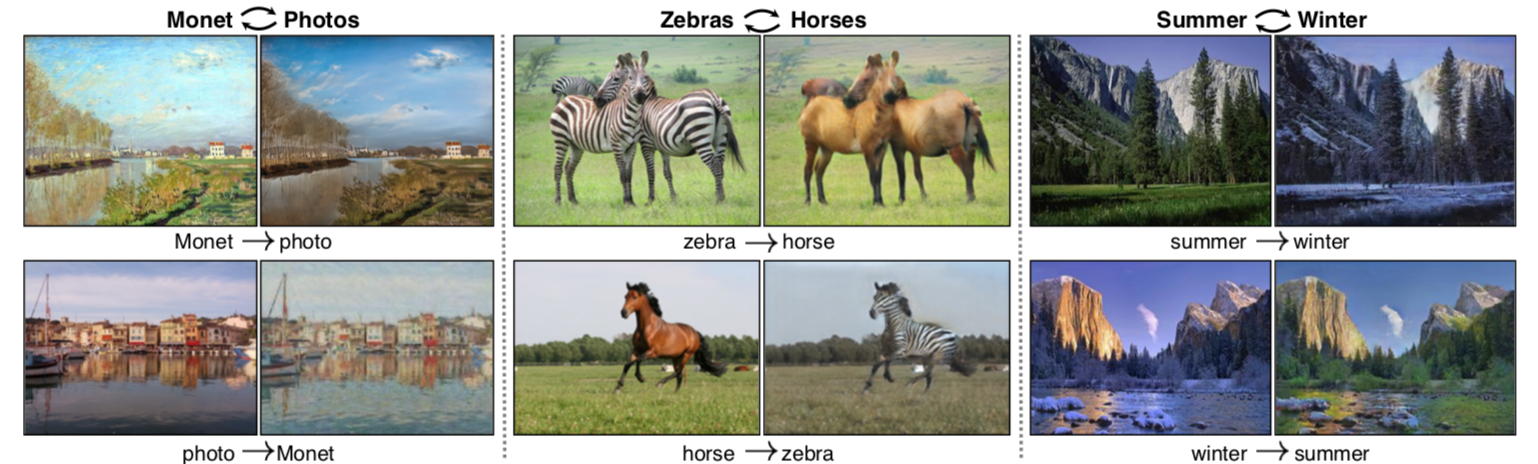
\includegraphics[width=\linewidth]{GAN/cyclegan_example}}
\caption{\label{fig:cyclegan_examples} \textbf{CycleGAN: Examples of translations between various domains.} Examples of bi-directional mappings between photography and Monet artworks, zebras and horses and summer and winter images. Figure reprinted from \cite{zhu_unpaired_2017}.}
\end{figure}

The model consists of two generators, $G_{X}$ and $G_{Y}$, which learn mapping from image domain $X$ to image domain $Y$, $G_{Y}: X \rightarrow Y$, and vice versa, $G_{X}: Y \rightarrow X$. Each of the image domains has its own discriminator, $D_{X}$ and $D_{Y}$, that check if the given image comes from the real distribution of the domain or is translated from the opposite domain.

\paragraph{Adversarial Loss}
The adversarial loss is applied to both pairs of networks, $(D_{X}, G_{X})$ and $(D_{Y}, G_{Y})$.
\begin{equation}
\mathcal{L}_{adv}(D_{X},G_{X}) = \mathbb{E}_{x}[\log D_{X}(x)] + \mathbb{E}_{y}[\log 1 - D_{X}(G_{X}(y))]
\label{eq:cyclegan_adv}
\end{equation}

\paragraph{Cycle Consistency Loss}
Additionally to the adversarial loss, CycleGAN also implements a so-called \emph{Cycle Consistency Loss}, which enforces that an image encoded from one domain to another, can also be reconstructed back to the original domain. The authors argue, that reducing the amount of possible mapping functions can help avoid the network to learn mappings that contradict each other \cite{zhu_unpaired_2017}.

The \textit{forward cycle consistency} defines that an image $x$ from domain $X$ and its encoded-decoded version should be approximately the same: $G_{X}(G_{Y}(x)) \approx x$. The \textit{backward cycle consistency} defines the same for an image from domain $Y$.
\begin{equation}
\mathcal{L}_{cyc}(G_{X},G_{Y}) = \mathbb{E}_{x}[||G_{X}(G_{Y}(x)) - x||_{1}] + \mathbb{E}_{y}[||G_{Y}(G_{X}(y)) - y||_{1}]
\label{eq:cyclegan_cycle}
\end{equation}


\begin{figure}[t]
\centering
\subcaptionbox{CycleGAN Model}
{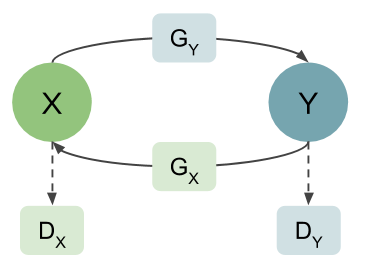
\includegraphics[height=4cm]{GAN/cyclegan1}}\hspace{1cm}
\subcaptionbox{Cycle Consistency Loss}
{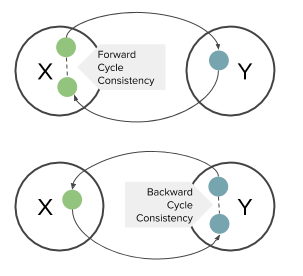
\includegraphics[height=4cm]{GAN/cyclegan2}}
\caption{\label{fig:cyclegan} \textbf{CycleGAN} (a) The model consists of two mappings, $G_{X}$ and $G_{Y}$ and corresponding discriminators $D_{X}$ and $D_{Y}$. (b) Cycle Consistency Loss measures the L1 distance between a real sample from one image domain and its encoded-decoded version. Figure adapted from \cite{zhu_unpaired_2017}.}
\end{figure}


\paragraph{Training Objective}
Both generators train to minimize and both discriminators train to maximize the final objective, which regulates the relative weight of the adversarial loss against the cycle consistency loss with the hyperparameter $\lambda$.
\begin{equation}
\begin{split}
G^{*}_{X}, G^{*}_{Y} = arg \ \underset{G_{X}, G_{Y}}{\mathrm{min}} \ \underset{D_{X}, D_{Y}}{\mathrm{max}} \ \mathcal{L}_{adv}(D_{X},G_{Y}) \ +  \mathcal{L}_{adv}(D_{Y}, G_{X}) \\ + \ \lambda \mathcal{L}_{cyc}(G_{X}, G_{Y})
\end{split}
\end{equation}

\paragraph{Architecture}
CycleGAN models are roughly based on Deep Convolutional GANs \cite{radford_unsupervised_2015}, using the PatchGAN architecture \cite{isola_image--image_2016} for the discriminator.


\pagebreak
% =======================================================================
\subsubsection{StarGAN}
% =======================================================================

One of the disadvantages of Pix2Pix and CycleGAN is the missing possibility of multi-domain translation. If there are more than 2 domains to translate between, one must train a new model for each domain pair. This can be time and computationally intensive.

StarGAN \cite{choi_stargan_2017} is unique among the tested models, as it is able to train one single generator that maps input to multiple domains, as shown in Figure \ref{fig:stargan_topo}. Using the conditional GAN model \cite{mirza_conditional_2014}, the generator is conditioned on a randomly chosen target domain each iteration, so that it can learn mapping for all given domains. %StarGAN does not require paired image examples, however, the images need to be labeled in order to be separated into different domains.

\begin{figure}[h]
\centering
\subcaptionbox{Cross-Domain Models}
{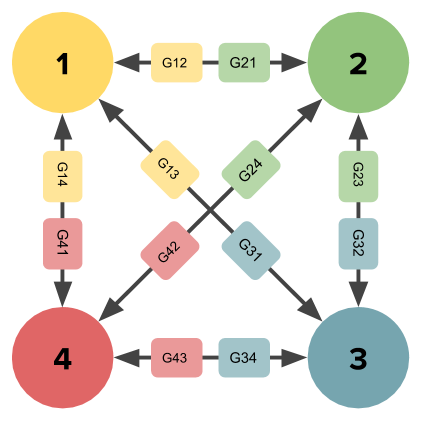
\includegraphics[height=4cm]{StarGAN_graph}}\hspace{1cm}
\subcaptionbox{StarGAN Model}
{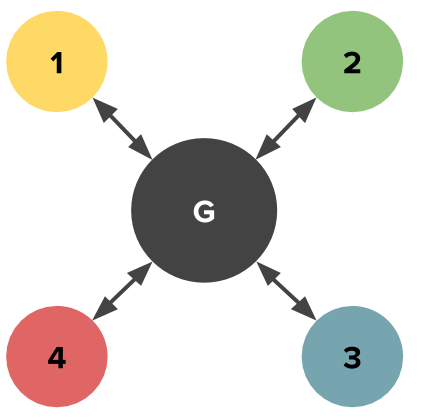
\includegraphics[height=4cm]{StarGAN_graph2}}
\caption{\label{fig:stargan_topo} \textbf{Comparison of cross-domain models and StarGAN model.} While cross-domain models need one generator per each domain pair, StarGAN only trains one generator for multiple domains. Figure adapted from \cite{choi_stargan_2017}.}
\end{figure}

The overall training objective of StarGAN consists of three loss functions:
\begin{itemize}
\item \textit{Domain Classification Loss}, which forces the discriminator to also output the domain class of the input image,
\item \textit{Adversarial Loss}, which is maximized by the discriminator and minimized by the generator,
\item \textit{Cycle Consistency Loss}, which measures the distance between an original image and its version encoded-decoded by the generator.
\end{itemize}

\begin{figure}[h]
\centering
{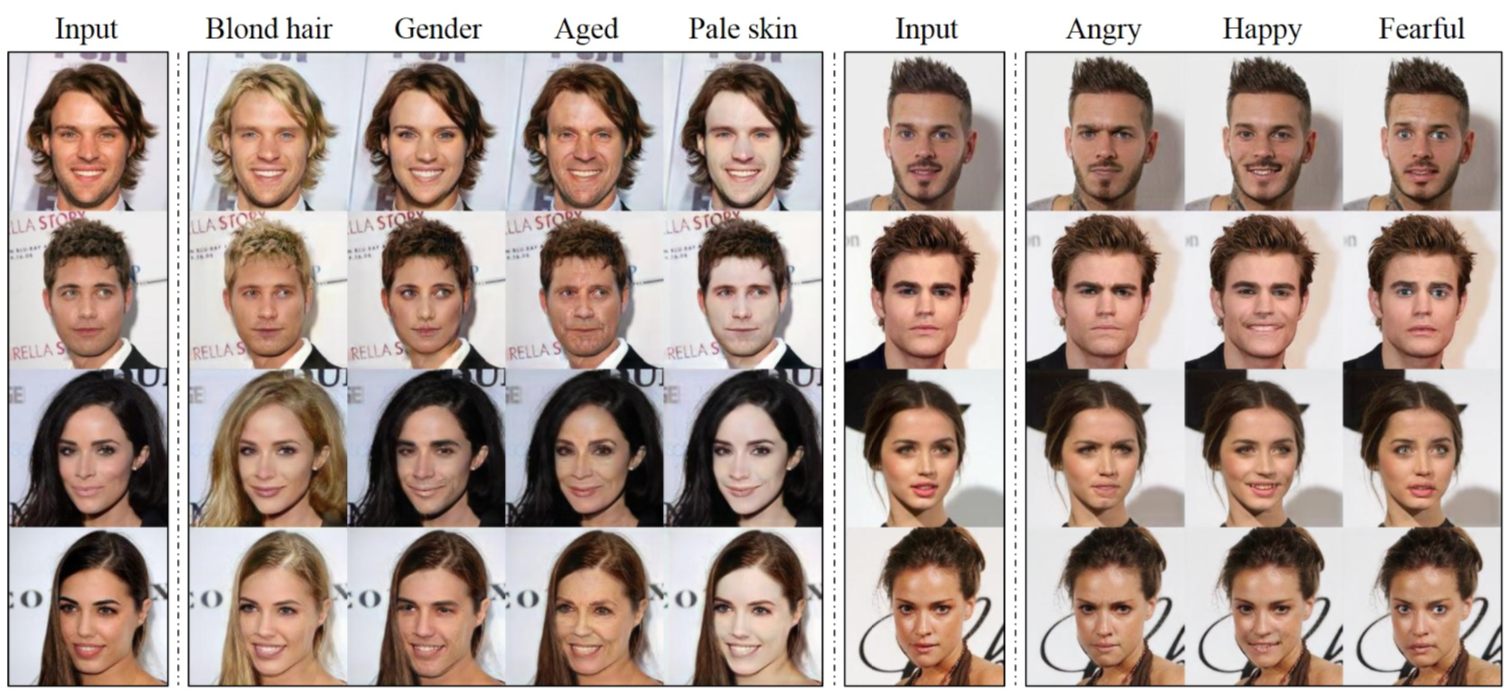
\includegraphics[width=\linewidth]{GAN/stargan_example}}
\caption{\label{fig:stargan_examples} \textbf{StarGAN: Examples of translations based on various attributes.} The first and sixth columns show the input image, the rest columns show modified versions based on the given attribute. Figure reprinted from \cite{choi_stargan_2017}.}
\end{figure}

\paragraph{Domain Classification Loss} 
Instead of feeding the target domain class $c$ to the discriminator, as in common conditional networks, StarGAN trains the discriminator to classify it. It uses an auxiliary classifier GAN, AC-GAN \cite{odena_conditional_2016}, which forces the discriminator to output both the probability distribution over the sources of the input, and the probability of the target domain labels, $D: x \rightarrow {D_{src}(x), D_{cls}(x)}$. This improves the network's stability and performance, as it forces the discriminator to perform and additional task.

This modification to the discriminator introduces the \textit{Domain Classification Loss} with two objectives, ${L}^{r}_{cls}$ and ${L}^{f}_{cls}$, optimizing $D$ and $G$ respectively. Given training data with an image $x$ and its original domain $c_{in}$, $D$ learns to classify the domain label correctly by minimizing the following objective:
\begin{equation}
\mathcal{L}^{r}_{cls} = \mathbb{E}_{x,c_{in}}[-\log D_{cls}(c_{in}|x)].
\label{eq:stargan_clsr}
\end{equation}

The generator objective is to generate images, that fool the auxiliary classifier and are classified as the target domain $c_{trg}$:
\begin{equation}
\mathcal{L}^{f}_{cls} = \mathbb{E}_{x,c_{trg}}[-\log D_{cls}(c_{trg}|G(x, c_{trg}))].
\label{eq:stargan_clsf}
\end{equation}


\paragraph{Adversarial Loss}
Given an image $x$ and a target domain label $c_{trg}$, generator $G$ tries to minimize the adversarial loss objective, to generate real-looking images conditioned on the target domain, while the discriminator classifying the source of the image, $D_{src}$, tries to maximize it.
\begin{equation}
\mathcal{L}_{adv} = \mathbb{E}_{x}[\log D_{src}(x)] + \mathbb{E}_{x, c_{trg}}[\log 1 - D_{src}(G(x, c_{trg}))]
\label{eq:stargan_adv}
\end{equation}

\paragraph{Cycle Consistency Loss}
Cycle Consistency Loss \cite{zhu_unpaired_2017} is used to generate images that preserve the underlying content of the original image, and only change the domain-related attributes:
\begin{equation}
\mathcal{L}_{cyc} = \mathbb{E}_{x,c_{in},c_{trg}}[||x - G(G(x,c_{trg}), c_{in})||_{1}].
\label{eq:stargan_cyc}
\end{equation}

\begin{figure}[h]
\centering
{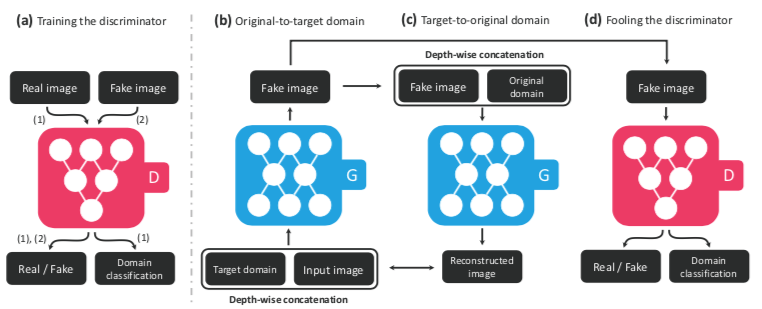
\includegraphics[width=\linewidth]{GAN/stargan}}
\caption{\label{fig:stargan_topo} \textbf{StarGAN Training Process.} The discriminator classifies the input as real or fake and outputs it's domain class prediction. The generator encodes the image with a target domain, and then decodes the output with the original domain, to calculate the cycle consistency distance. Figure reprinted from \cite{choi_stargan_2017}.}
\end{figure}

\paragraph{Training Objective}
The full training objective for $D$ and $G$ respectively is:
\begin{equation}
\mathcal{L}_{D} = -\mathcal{L}_{adv} + \lambda_{cls} \mathcal{L}^{r}_{cls},
\label{eq:stargan_D}
\end{equation}
\begin{equation}
\mathcal{L}_{G} = \mathcal{L}_{adv} + \lambda_{cls} \mathcal{L}^{f}_{cls} + \lambda_{cyc} \mathcal{L}_{cyc},
\label{eq:stargan_G}
\end{equation}

where $\lambda_{cls}$ and $\lambda_{cyc}$ control the relative importance of the two loss functions against the adversarial loss.

The model architecture is based on CycleGAN.


\pagebreak
% ==============================================================
\subsubsection{MUNIT}
% ==============================================================

All of the introduced models approach the image translation problem as one-to-one mapping. However, many of the image domain translation tasks are in fact multi-modal, meaning one single input can have multiple different outputs. The MUNIT network \cite{huang_multimodal_2018} introduces an unsupervised multi-modal method, which is able to capture the diversity of the output, as shown in Figure \ref{fig:munit_example}.

Instead of using translation in pixel space, the model tries to model the translation in a latent space. Based on the \textit{partially shared latent space assumption}, a content latent code $c \in \mathcal{C}$ and a style latent code $s_{i} \in \mathcal{S}_{i}$ are separated, assuming that the two image domains share a common content space but each has an individual style space. 

\begin{figure}[h]
\centering
{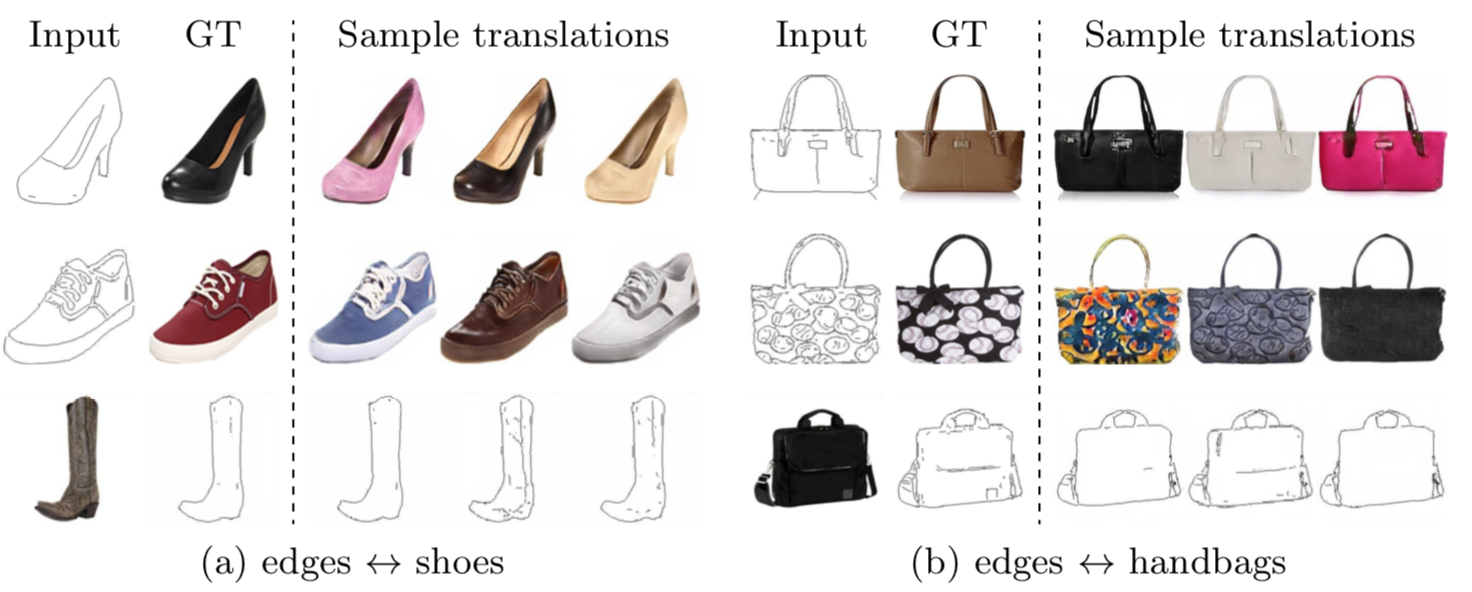
\includegraphics[width=\linewidth]{GAN/munit_example}}
\caption{\label{fig:munit_example} \textbf{MUNIT: Examples of multi-modal translations.} For both translations, the input and ground-truth image are shown in the first two columns and the rest shows various generated samples. Figure reprinted from \cite{huang_multimodal_2018}.}
\end{figure}


For each domain, there is an auto-encoder, which consists of a generator $G$ and two encoders: content encoder $E^c$, and style encoder $E^s$. Given an image $x \in X$, it is encoded into a content and style code, $E^c_x(x)$ and $E^s_x(x)$. To translate the image $x \in X$ to domain $Y$, its content code $c_{x}$ is extracted using the content encoder $E^c_x$, and it is combined with a random style code $s_{y}$, $G_y(c_x, s_y)$. 

While the style code is assumed to have a global and simple effect and is therefore sufficiently represented by a low-dimensional vector, the content is assumed to be a high-dimensional vector describing the complex spatial structure of the data. Figure \ref{fig:munit_enc} shows the encoding of an image from domain $X$ to style and content code and the decoding back to the image domain.

\begin{figure}[h]
\centering
{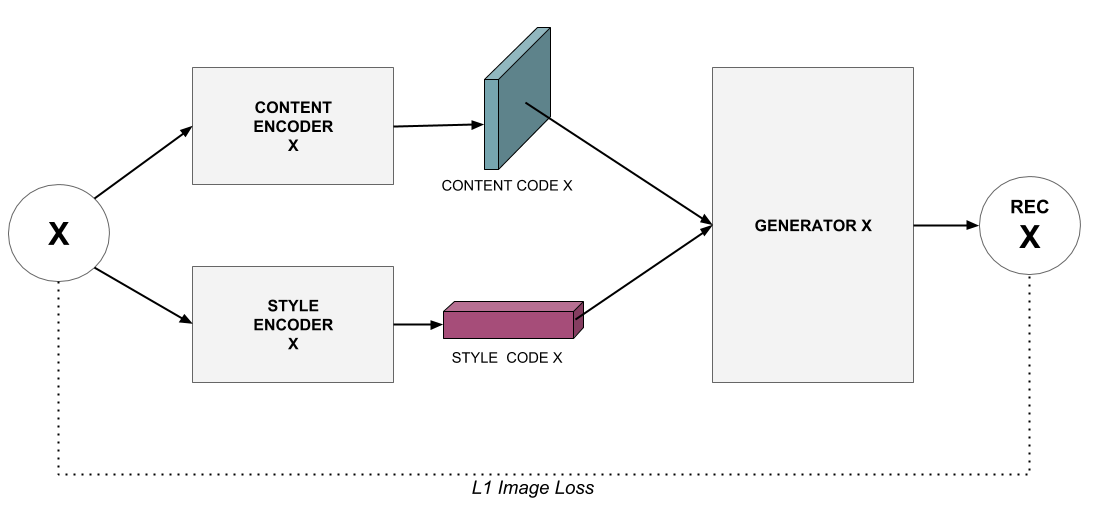
\includegraphics[width=\linewidth]{GAN/munit_enc}}
\caption{\label{fig:munit_enc} \textbf{MUNIT within-domain reconstruction.}  An image from domain X is decomposed into content and style code via respective encoders. The decoder is a generator that combines the two latent encodings and translates them back to the original domain. A reconstruction loss is calculated between the original and the reconstructed image to optimize the auto-encoders. Figure adapted from \cite{huang_multimodal_2018}.}
\end{figure}

\paragraph{Reconstruction Loss}
The reconstruction loss is similar to the cycle consistency loss \cite{zhu_unpaired_2017}, enforcing the reconstruction between an image and its latent representation in both directions. 

The \textit{image reconstruction loss} encourages the reconstruction of an image after encoding to latent space and decoding back to image space.
\begin{equation}
\mathcal{L}^{x}_{rec} = \mathbb{E}_{x}[||x - G_{x}(E^{c}_{x}(x), E^{s}_{x}(x))||_{1}]
\end{equation}

The \textit{latent reconstruction loss} consists of a style loss and a content loss, which should be reconstructed after being encoded to image space and decoded back. The content loss enforces the preservation of semantic information of the translated image, while the style loss encourages diversity in the translated outputs.
\begin{equation}
\mathcal{L}^{c_{x}}_{rec} = \mathbb{E}_{c_{x}, s_{y}}[||c_{x} - E^{c}_{y}(G_{y}(c_{x},s_{y}))||_{1}]
\end{equation}
\begin{equation}
\mathcal{L}^{s_{y}}_{rec} = \mathbb{E}_{c_{x}, s_{y}}[||s_{y} - E^{s}_{y}(G_{y}(c_{x},s_{y}))||_{1}]
\end{equation}

The same losses are also applied to image domain $Y$.

\begin{figure}[h]
\centering
{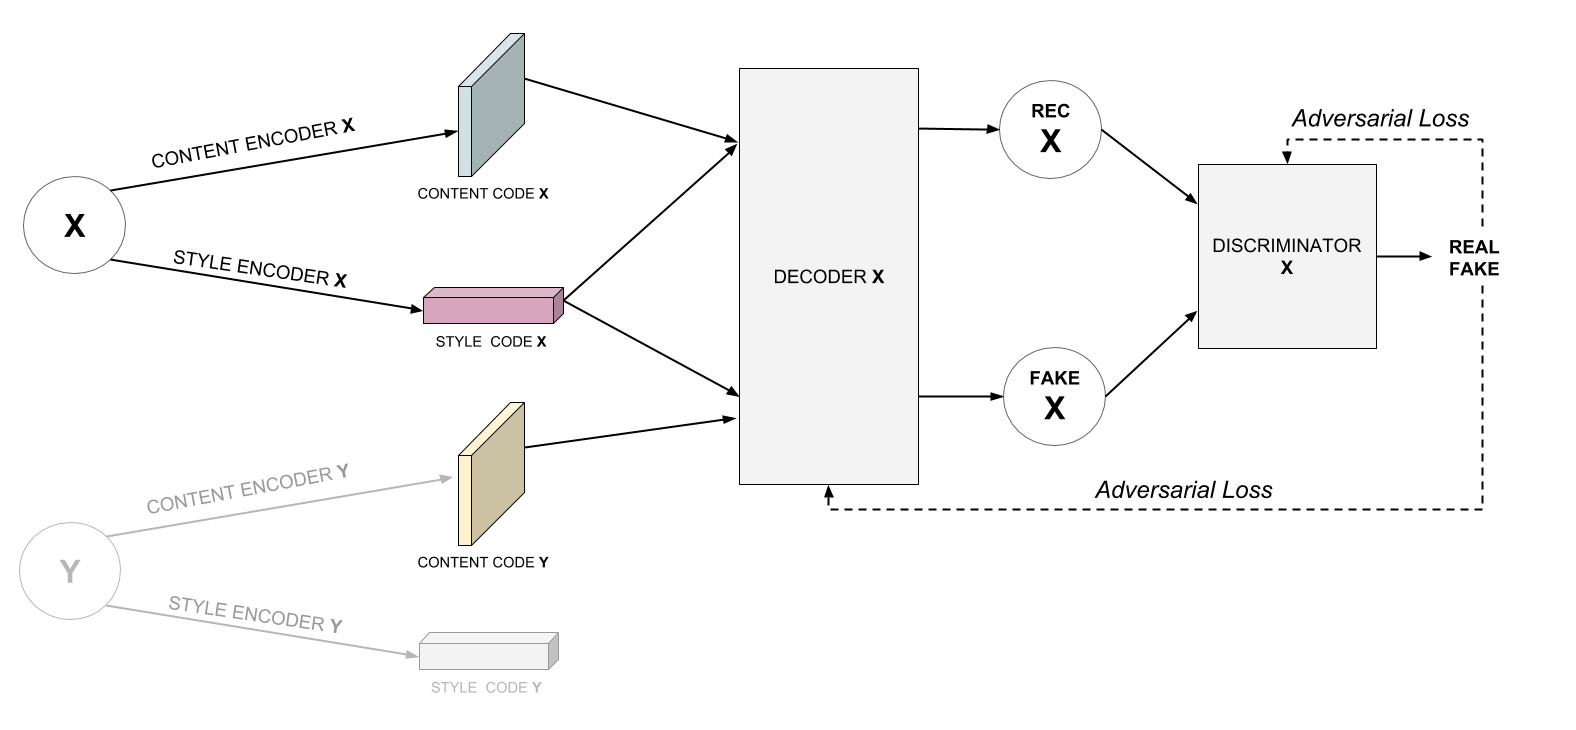
\includegraphics[width=\linewidth]{GAN/munit_adv}}
\caption{\label{fig:munit_adv} \textbf{MUNIT cross-domain translation.} The content code of image from domain Y is combined with style from domain X to generate a fake image X. The discriminator decides if the image was translated or comes from the original image domain based on which the adversarial objective is calculated. Figure adapted from \cite{huang_multimodal_2018}.}
\end{figure}

\paragraph{Adversarial Loss}
In order to enforce the generated output to look realistic, each domain has a discriminator, $D_x$ and $D_y$, which is trained to distinguish if the source of the image is the data distribution of the image domain, or if it was generated by the auto-encoder.
\begin{equation}
\underset{G_x}{\mathrm{min}} \ \underset{D_x}{\mathrm{max}} \ \mathcal{L}^{x}_{adv} = \mathbb{E}_{x}[logD_{x}(x)] + \mathbb{E}_{c_{y}, s_{x}}[log(1 - D_{x}(G_{x}(c_{y}, s_{x})))]
\end{equation}

Figure \ref{fig:munit_adv} shows the adversarial loss for translation from domain $Y$ to domain $X$. The adversarial loss for domain $Y$ is defined similarly.


\paragraph{Training Objective}
The overall training objective, which is trained to be maximized by the discriminators and minimized by the generators and auto-encoders can be modified by $\lambda$, $\lambda_c$, $\lambda_s$, controlling the relative weight of each loss:
\begin{equation}
\underset{G_x, G_y, E_x, E_y}{\mathrm{min}} \ \underset{D_x, D_y}{\mathrm{max}} \ \mathcal{L} = \mathcal{L}^{x}_{adv} + \mathcal{L}^{y}_{adv} + 
\lambda(\mathcal{L}^{x}_{rec} + \mathcal{L}^{y}_{rec}) + 
\lambda_c(\mathcal{L}^{c_x}_{rec} + \mathcal{L}^{c_y}_{rec}) + 
\lambda_s(\mathcal{L}^{s_x}_{rec} + \mathcal{L}^{s_y}_{rec})
\end{equation}


\pagebreak
% ==============================================================
\subsubsection{Fader Networks}
% ==============================================================
The Fader Networks \cite{lample_fader_2017} is an unsupervised technique of training GANs that, similarly to MUNIT \cite{huang_multimodal_2018}, translates images in latent space instead of pixel space. 

The unique feature of Fader Networks is that the images are modified based on attribute values that are regarded as continuous, e.g: the network can translate a photo of a young person to old person at increasing level of interpolation. Figure \ref{fig:fader_ex} shows example interpolations of different attributes.

Similarly to MUNIT \cite{huang_multimodal_2018}, the model consists of an encoder-decoder architecture, which learns how to translate an input image to its latent representation, and a discriminator to enforce an adversarial approach. In case of Fader Networks the latent representation is a $N$-dimensional vector $z$.

\begin{figure}[h]
\centering
{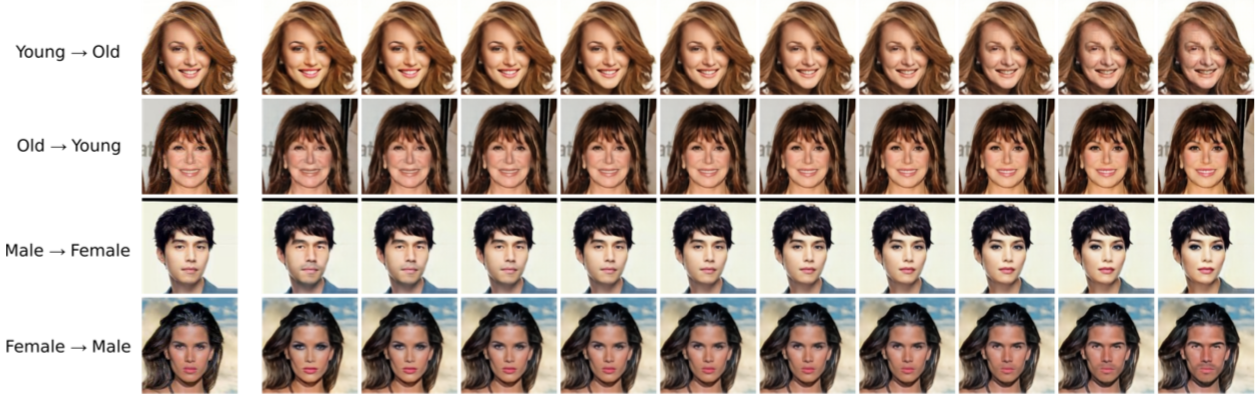
\includegraphics[width=\linewidth]{GAN/fader_example}}
\caption{\label{fig:fader_ex} \textbf{FaderNetworks: Interpolations of different attributes.} The original image on the left is translated to the given attribute with increasing intensity from left to right. The outputs of the decoder and discriminator are compared to ground truth and the networks parameters are optimized accordingly. Figure reprinted from \cite{lample_fader_2017}.}
\end{figure}


Given a pair of input image and its corresponding attribute ($x^i \in X, y^i \in Y$), the encoder maps it to its latent representation $z$, $Enc: X \rightarrow \mathbb{R}^N$. The decoder takes a latent vector $z$ and a target attribute $y'$, and translates it to a modified version of the image, $Dec: (\mathbb{R}^N, Y) \rightarrow X$.

The essential feature of this approach is that latent representation of an image is \textit{attribute-invariant}, e.g: an image of the same person young and old should be encoded as the same latent vector. Without this invariance, the decoder would simply learn to ignore the given attribute value. By removing the information about the attributes from the encoded representation, the decoder must consider the attribute in order to reconstruct the image.

However, since paired image training data is not available, the invariance cannot be enforced by adding a simple distance to the loss function, instead it must be learned through an adversarial objective on the latent space. Therefore, the architecture also includes a discriminator network $Dis$, which is trained to predict the attribute value $y$ of an image $x$, given its latent representation $E(x)$.

\begin{figure}[h]
\centering
{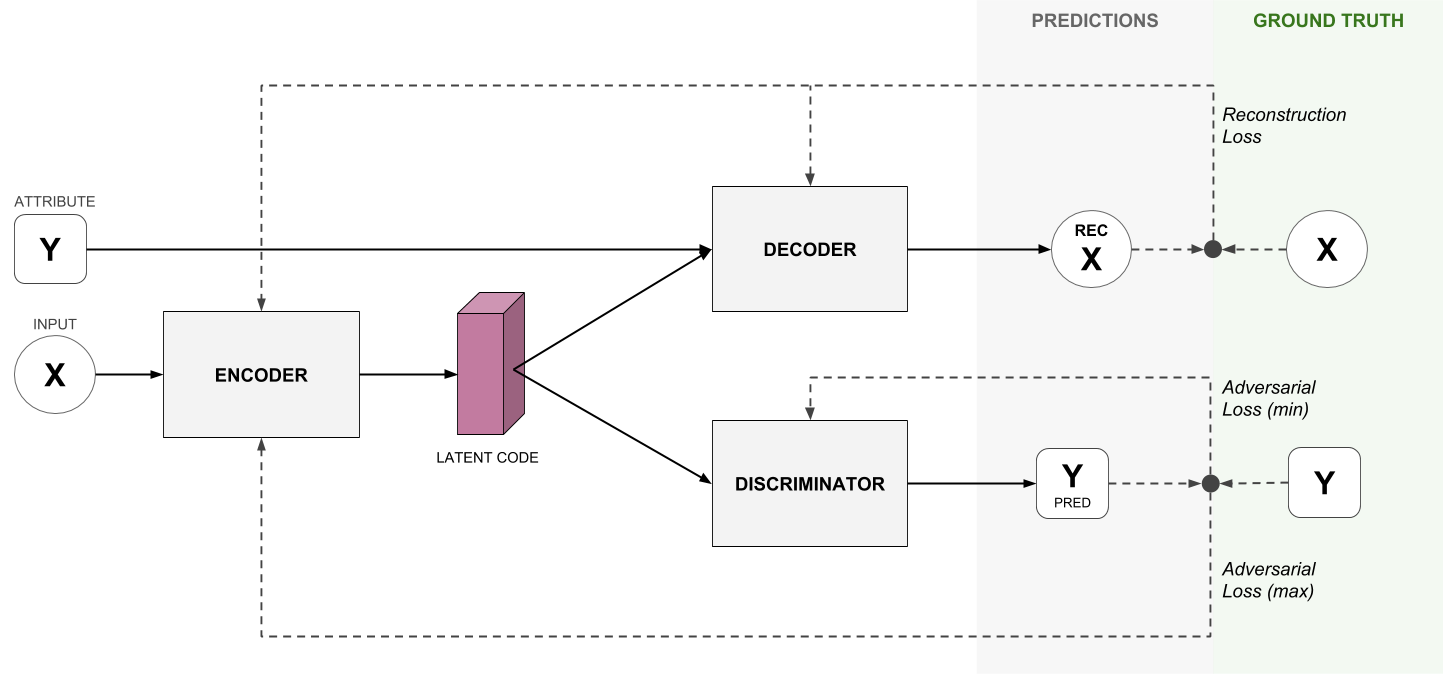
\includegraphics[width=\linewidth]{GAN/fader}}
\caption{\label{fig:fader_ex} \textbf{FaderNetworks Model.} Given a training pair of input image and attribute value, the image is encoded to a latent code. The decoder learns to reconstruct the image based on its latent code and attribute value, while the discriminator tries to predict the attribute based on the latent code. Figure adapted from \cite{lample_fader_2017}.}
\end{figure}


\paragraph{Reconstruction Loss}
The authors use a \textit{mean squared error} loss (MSE) to optimize the auto-encoder to output images similar to the original inputs. However, they mention that the previously described \textit{PatchGAN} architecture with L1 loss might lead to sharper results.
\begin{equation}
\mathcal{L}_{rec}(Enc,Dec) = \mathbb{E}_{x,y}[||x-Dec(Enc(x),y)||^2_2]
\end{equation}

\paragraph{Adversarial Loss}
The discriminator trains to predict the attributes correctly:
\begin{equation}
\mathcal{L}_{Dis} = \mathbb{E}_{x,y}[log(Dis(y|Enc(x)))],
\end{equation}

while the objective of the encoder is for the decoder to be able to reconstruct the image, and to prevent discriminator from correct classification:
\begin{equation}
\mathcal{L} = \mathcal{L}_{rec} - \lambda_E \mathbb{E}_{x,y}[log(Dis(1-y|Enc(x)))].
\end{equation}


\pagebreak
% ==============================================================
\subsection{Image Retrieval Features}
% ==============================================================



\subsubsection{Akiwi}
The Akiwi website \cite{sonnenberg_akiwi_nodate} provides an API, where user can upload an image file and the API returns a feature vector which can be used as the image descriptor to compare similarities with other image features.

The API provides various descriptors: the 50-dimensional feature is based on low-level feature descriptors such as a color histogram and edge detection of the image. The 64-dimensional feature is a feature produced by the last hidden layer of a ResNet network, which was normalized and reduced to 64 dimensions \cite{Barthel:2017:VBM:3078971.3079016}.


\subsubsection{ResNet}
Nowadays, almost every deep learning framework offers a variety of pre-trained convolutional networks. The deep learning framework PyTorch offers 6 different pre-trained CNN architectures, such as the \textit{VGG Network} \cite{simonyan_very_2014}, \textit{Inception Network} \cite{szegedy_rethinking_2015} or the \textit{ResNet} \cite{he_deep_2015}. 

The networks are pre-trained to classify images from the ImageNet dataset, which contains around 14 million images labels with 1.000 classes, and has established itself as a reference for testing convolutional architectures. 

Currently, the best scoring pre-trained model offered by PyTorch is the \textit{ResNet152}, which is 152 layers deep and contains so-called \textit{Residual Blocks}. These blocks allow the output of one layer to be added directly to another layer deeper in the network. This technique is useful when training very deep neural networks.

\begin{figure}[h]
\centering
{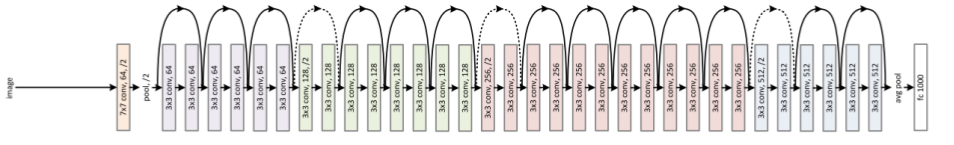
\includegraphics[width=\linewidth]{CBIR/resnet_arch}}
\caption{\label{fig:search_pink} \textbf{Resnet34 Architecture.} An example of the ResNet architecture with 34 layers. Figure reprinted from \cite{noauthor_resnet-152_nodate}}.
\end{figure}

The extraction of the image feature happens at the last hidden layer of the network, which in case of ResNet152, is a 2048-dimensional layer. For each image, the output of this layer is its unique descriptor, which can be used to compare distances between images.

Since the ResNet152 was trained on a dataset with a big variety of objects, most of the product images most likely fall to one category and therefore could have very similar feature vectors, which do not magnify the differences between the products enough.

Training of such a deep network from scratch can be very time consuming and requires a big enough dataset. Therefore I used the so-called \textit{Transfer Learning}, where one can use a network trained on a big dataset, such as the ImageNet dataset, and only re-train the last few layers of the network to classify a new dataset.

I re-trained the network's last hidden layer on the fashion dataset, to classify the 7 categories of the products, such as blouses, dresses, pants etc. 


\pagebreak
% ==============================================================
\section{Experiments}
% ==============================================================
The objective of the experiments is to improve image retrieval of fashion products, by allowing the user to perform a series of modifications on the given product image. Unless indicated differently, the experiments were performed on the data category of dresses to reduce the complexity of the experiments and the algorithms and simplify the evaluation process.

The experiments were conducted in \textit{Python 3} \cite{noauthor_welcome_nodate}, using the machine learning framework \textit{PyTorch} \cite{noauthor_pytorch_nodate} and several common python packages, such as: \textit{pandas} \cite{noauthor_python_nodate}, \textit{numpy} \cite{noauthor_numpy_nodate}, \textit{scikit-learn} \cite{noauthor_scikit-learn_nodate}, \textit{matplotlib} \cite{noauthor_matplotlib_nodate}, \textit{PIL} \cite{noauthor_pillow_nodate} and others. 

%TODO train / val / test split


% ==============================================================
% PRODUCTS TO MODLES
% ==============================================================
\pagebreak
\subsection{Products to Models Translation}
Most fashion online stores provide product images that are taken on white background without a person modeling the product. However, there are also countless images online, coming from social media, blogs and other platforms, of people wearing a certain product, without a corresponding product image. 

The goal of this experiment was to translate a product image to an image of a person wearing that product, in order to be able to extend the search possibilities.

I have first experiment with the MUNIT network - an unsupervised approach, translating between the domain of all product images and the domain of all model images. This approach has not yielded the desired results, since the output was too diverse and it failed to represent the input product.

Therefore I have decided to train the network in a supervised manner, such that it learns to map an image of a specific product to an image of a model wearing that specific product. This task required a dataset consisting of image pairs, which I created using a clustering algorithm.

\pagebreak
\subsubsection{Data Clustering}
As mentioned in Section \ref{sec:data}, each scraped product has a variable amount of images displaying people modeling the given product. The average amount of images for a product is 4, and based on manual screening of the dataset, these images follow a certain pattern: full-body model front-facing, full-body model back-facing, zoom to part of body were product is worn and large zoom on detail.

In order to create a dataset of image pairs, each product must have exactly one corresponding model image. I chose the most common and basic model image - where the model is facing the camera and the full body is captured. 

However, there is no clear order or pattern from which to deduce the pose of the model based on the name of the image or its position in the list of images. Since there are more than 60.000 model images only for category dresses, manual selection of the best image for each product would be too time consuming.

To identify the best image for each product, I used the following approach:
\begin{enumerate}
	\item \textbf{Image Processing}: Highlight most relevant features, such as contours, while suppressing irrelevant features, such as color.
	\item \textbf{Clustering}: Cluster features and experiment with amount of clusters.
	\item \textbf{Select Best Cluster}: Visualize clusters and manually select the best cluster center.
	\item \textbf{Select Best Image}: For each product, select the image with the smallest distance to the best cluster center.
\end{enumerate}


For clustering, I used the \textit{K-Means Clustering} algorithm \cite{noauthor_k-means_2018}, which creates $k$ clusters and assigns each data point to the nearest cluster center. The \textit{scikit-learn} library offers a fast implementation of the algorithm \cite{noauthor_sklearn.cluster.kmeans_nodate}.

\paragraph{Grayscale Clustering}
Since most of the models are photographed on a white background, for the initial experiment, I have converted the images to grayscale, in order to separate the person from the background regardless of the color.

In order to reduce the dimensionality and speed up the algorithm, I resized the images to $64\times64$ pixels. The total number of model images is $63.103$, which means the clustering algorithm was fed with an array of size $63103\times64\times64$.

\begin{figure}[h]
\centering
{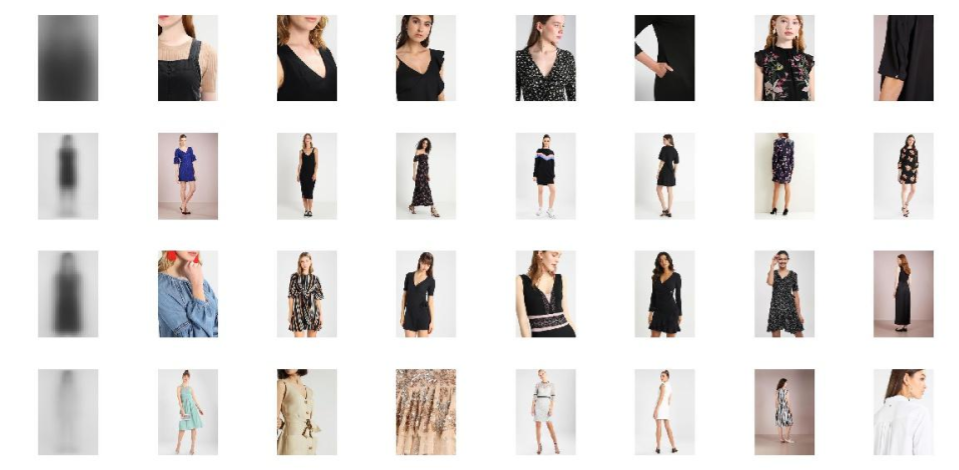
\includegraphics[width=\linewidth]{clustering/grayscale}}
\caption{\label{fig:cluster_gray} \textbf{Cluster centers with grayscale features.} Each row displays one cluster center (left-most image) and random images from the dataset that are assigned to the respective cluster center based on their grayscale feature vector.}
\end{figure}

Figure \ref{fig:cluster_gray} shows the results of K-Means clustering with 4 cluster centers. The second cluster center seems to be the most suitable to find front-facing full-body images. However, as one can see from the results, the fourth cluster center tends to group all images with light-colored dresses, in all poses. 

Therefore grayscale features do not fit the requirement for the clustering process to disregard color as a feature.


\paragraph{Edges}
In order to avoid the problem of separating dark and light colors into different clusters, I used the \textit{Canny Edge Detection} algorithm on the model images. This feature only considers the contours of the object in the image and is invariant to color.

As part of the data collection process, all images were resized to a uniform size of $256\times256$, extending the shorter side with white color. However, some models are photographed on a darker background and the edge detection algorithms can detect this transition of light-grey background to white as an edge.

Some clustering experiments were affected by this detection and tended to group images with darker backgrounds together, regardless of the model pose. Therefore, in all further experiments, the images have center-cropped width of 116 pixels.

\begin{figure}[h]
\centering
{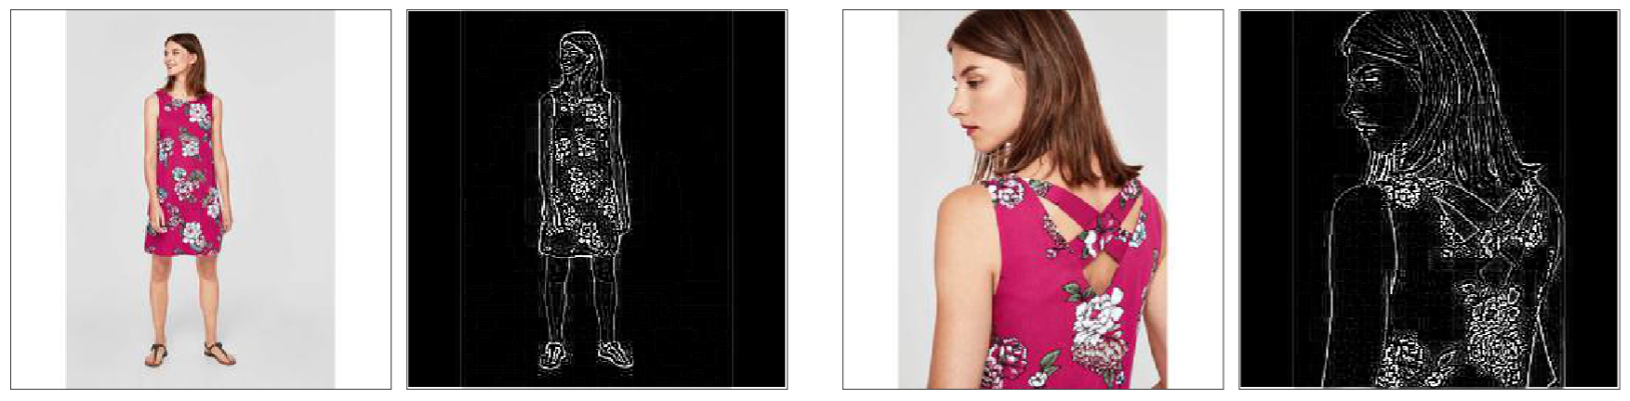
\includegraphics[width=\linewidth]{clustering/edges_data}}
\caption{\label{fig:cluster_edges_data} \textbf{Canny Edge Detection for model images.} Each left image shows original image and right image shows the corresponding edges produced with Canny Edge detection algorithm.}
\end{figure}

Overall, clustering with edges did not prove to be effective, as the edges are very thin and therefore the measured distance between two images, which are quite similar, but a little bit shifted, would be very big. The detection is also quite sensitive to patterns in the dresses, as seen in Figure \ref{fig:cluster_edges_data}.

\paragraph{Threshold Mask}
To avoid the difficulties with thin edges, I applied a thresholding technique to the images, in order to fill the person's contour with white color and background with black. Figure \ref{fig:cluster_outline_data} shows the steps applied to each image to get a binary threshold mask.

\begin{figure}[h]
\centering
{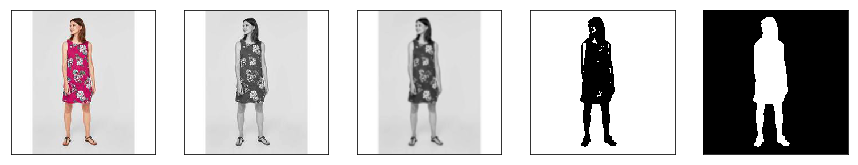
\includegraphics[width=\linewidth]{clustering/outlines_data}}
\caption{\label{fig:cluster_outline_data} \textbf{Threshold Mask for model images.} Starting from left is the original image, converted to grayscale, applied Gaussian blur, binary threshold, and the image masked with binary threshold.}
\end{figure}

This feature selection has proven to be the most effective for \textit{K-Means} algorithm with 3 cluster centers. First column of Figure \ref{fig:cluster_outline} shows the three cluster centers: the first groups full-body photographs, second groups zoomed images of upper-body and the last one groups detail images. 

\begin{figure}[h]
\centering
{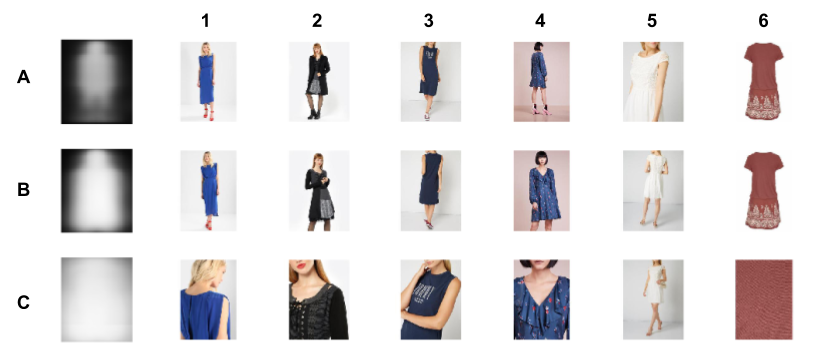
\includegraphics[width=\linewidth]{clustering/outlines_clusters}}
\caption{\label{fig:cluster_outline} \textbf{Cluster centers with threshold mask.} The rows A-C show 3 cluster centers created by \textit{K-Means Clustering} algorithm with threshold mask features of images. Each column $1-6$ shows one product and the image that is closest to the respective cluster center.}
\end{figure}

Each row of Figure \ref{fig:cluster_outline} shows the image that is the closest to the respective cluster center for the given product 1-6. The products can have more photographs that are not displayed because they are not the best match for any of the cluster centers, as well as  one photograph can be best match for more than one cluster center. 

We can observe that products $1-4$ are grouped accordingly to expectations. Product $5$ is problematic, because the dress is lighter than the background, so its features do not match the cluster centers as expected. Product $6$ is an example of an outlier product, where there are no model images available and instead only a product image is provided.

Figure \ref{fig:cluster_outline_distances} shows all available images for product 1 sorted based on their respective distances to cluster center \textbf{A}. The first picture is therefore the best match for the cluster center.

\begin{figure}[h]
\centering
{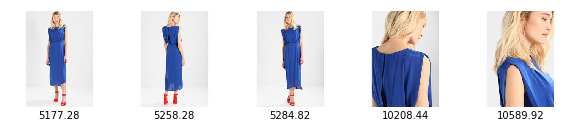
\includegraphics[width=\linewidth]{clustering/outlines_distances}}
\caption{\label{fig:cluster_outline_distances} \textbf{Product images distances to cluster center A.} Images are sorted by the distances towards cluster center A from Figure \ref{fig:cluster_outline}.}
\end{figure}

Based on these results, I selected cluster center \textbf{A} from Figure \ref{fig:cluster_outline} as the best and for each product chose the image which is closest to that center. Although there are some outliers in the results, the network working with this data should be able to learn to ignore them.

% --------------------------------------------------------------------------------------------
\pagebreak
\subsubsection{Supervised Training}
The only network from the evaluated models that translates images in a supervised matter is Pix2Pix \cite{isola_image--image_2016}. I have modified the official PyTorch implementation of the paper \cite{noauthor_junyanz/pytorch-cyclegan-and-pix2pix_nodate}, in order to work with the fashion data structure: \hyperlink{https://github.com/sonynka/pytorch-CycleGAN-and-pix2pix}{github.com/sonynka/pytorch-CycleGAN-and-pix2pix}.

Figure \ref{fig:pix2pix_arch} describes the used architecture of the network. In all experiments, I have used image size 256 and batch size 8. The learning rate starts at 0.0002 and is decreased gradually towards 0 throughout the training. Both networks are optimized using Adam optimizer. Most of the experiments were trained for around 20 hours.

\begin{figure}[h]
\centering
\subcaptionbox{Discriminator}{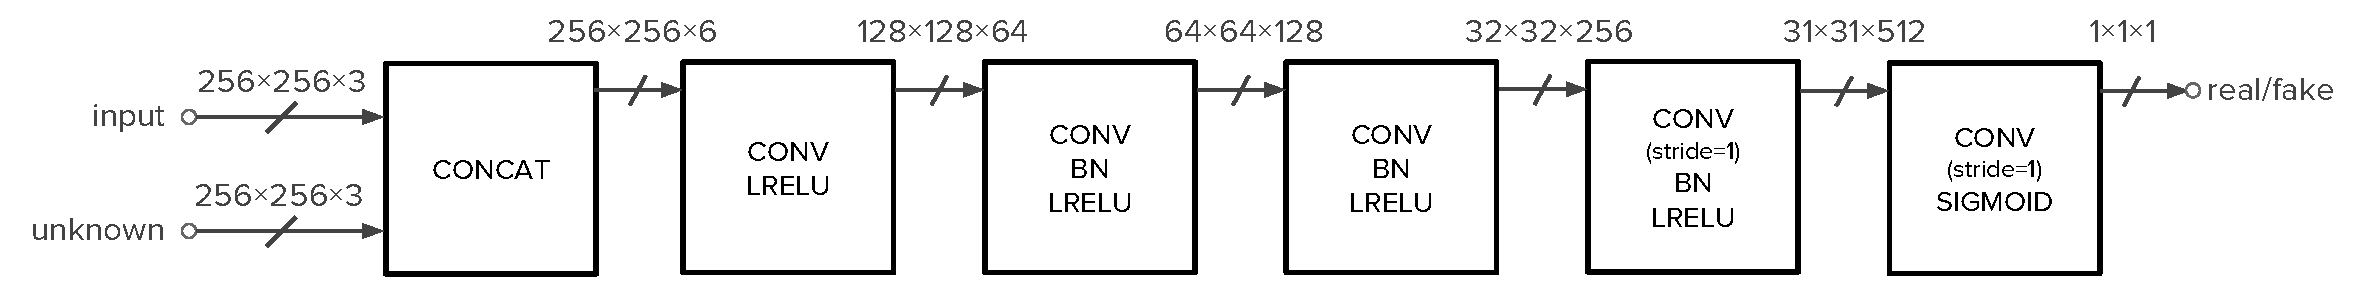
\includegraphics[height=1.5cm]{pix2pix/dis_arch}}\vspace{.5cm}
\subcaptionbox{Generator}{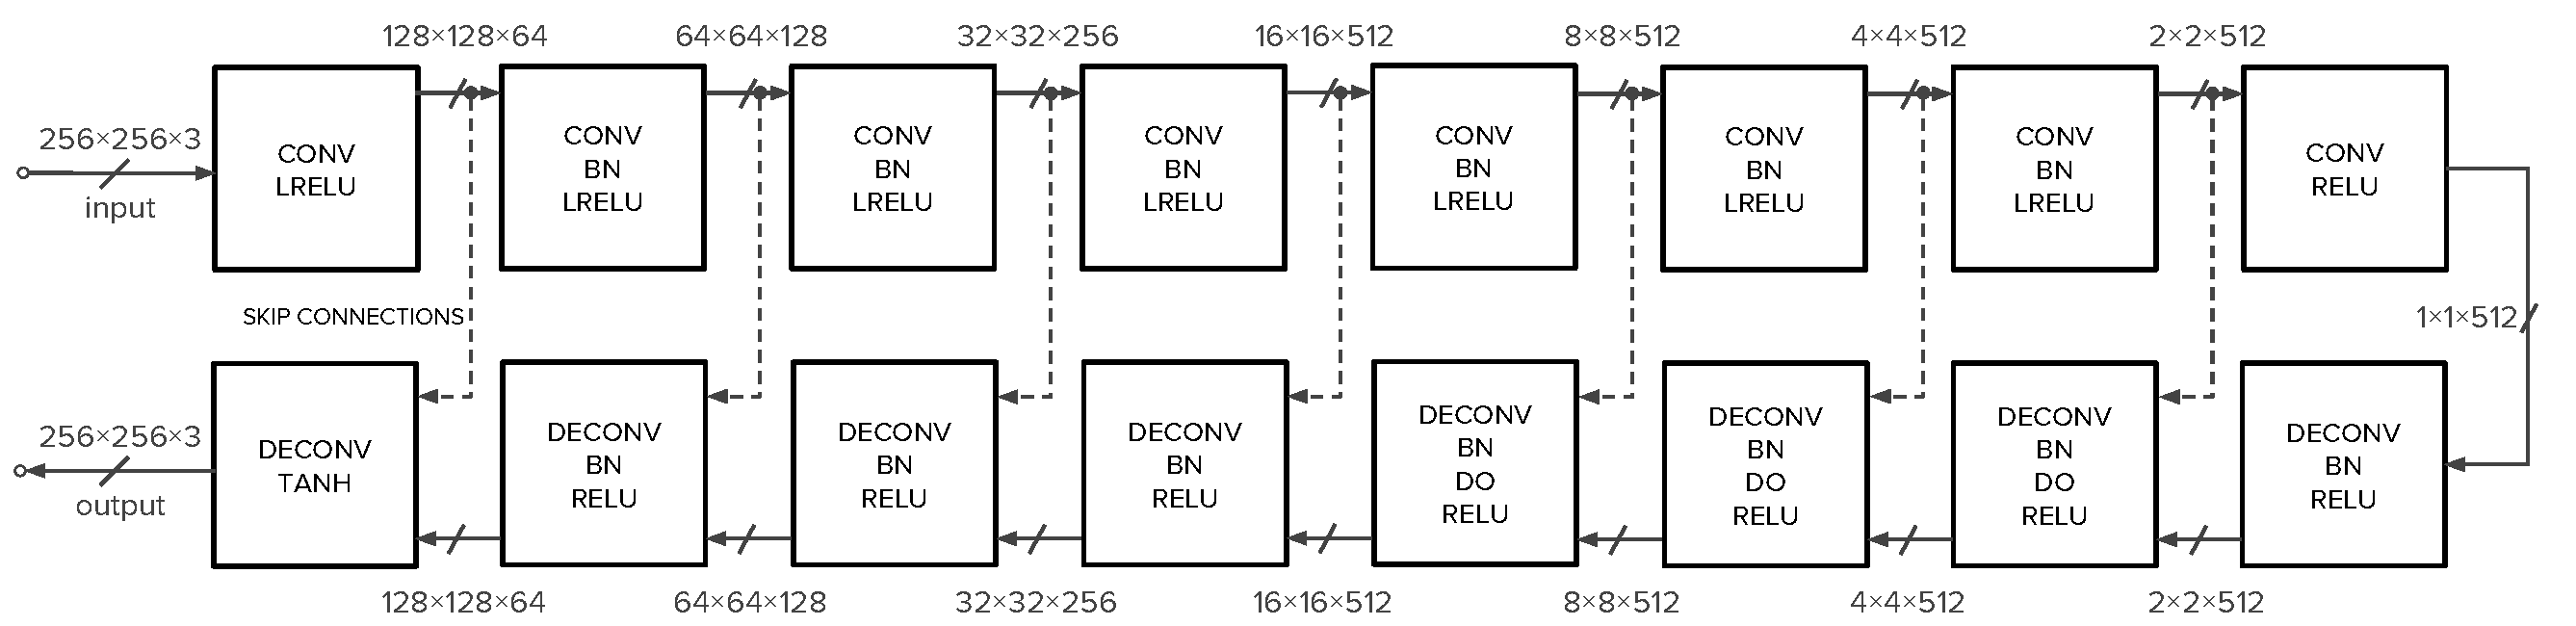
\includegraphics[width=\linewidth]{pix2pix/gen_arch}}
\caption{\label{fig:pix2pix_arch} \textbf{Pix2Pix Architecture.} The architecture of the trained  discriminator and generator. CONV denotes a convolutional layer with kernel size 4 and stride 2 unless indicated otherwise, BN denotes batch normalization, LRELU denotes leaky relu with slope 0.2 and DO denotes drop out with rate 50\%. Figure adapted from \cite{hesse_image--image_2017}.}
\end{figure}

\pagebreak
Training with the original set-up of the network resulted in a common GAN failure, discussed in Section \ref{sec:gan_diff}: the discriminator learns to distinguish the source of an image confidently too fast, resulting in the generator not having opportunity to improve. This behavior can be observed in Figure \ref{fig:pix2pix_losses}a, where the generator loss keeps growing throughout the training, while discriminator loss is minimized early on.

To avoid this issue, I added some noise to the labels to confuse the discriminator and give the generator and advantage in the training. In my implementation, the real labels fluctuate between 0.7 to 1.2 and fake labels can be anywhere between 0.0 and 0.3 \cite{chintala_starter_2018}. I also flipped the labels for the discriminator on cca 5 out of 100 iterations. As shown in Figure \ref{fig:pix2pix_losses}b, by disadvantaging the discriminator, both losses get stabilized.

\begin{figure}[t]
\centering
\subcaptionbox{Original Model}{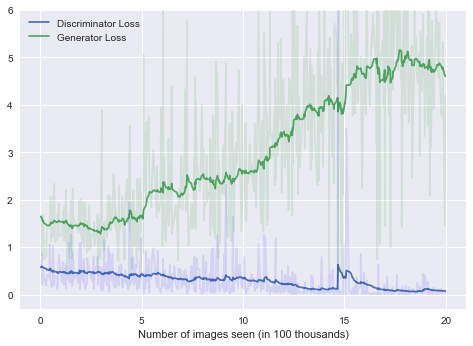
\includegraphics[width=.48\linewidth]{pix2pix/loss_original}}
\subcaptionbox{Label Noise}{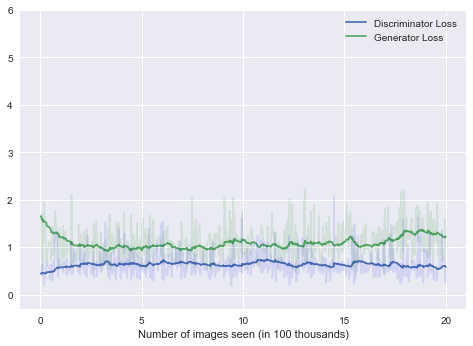
\includegraphics[width=.48\linewidth]{pix2pix/loss_soft_labels}}
\caption{\label{fig:pix2pix_losses} \textbf{Pix2Pix Adversarial Loss.} Adversarial loss of the discriminator and the generator, a) with the original pix2pix set-up, b) with adding noise to discriminator. For visualization purposes, the curves are smoothed, such as described in \cite{noauthor_tensorflows_2018}. The real loss values are shown in the background.}
\end{figure}

Although the learning curves can provide an inisight into the staibility of the training, there is no objective method to correlate the losses to whether the results look realistic - the network's outputs need to be evaluated mostly visually \cite{preserve_knowledge_how_nodate}. 

Figure \ref{fig:pix2pix_results} shows the generated samples from the test set for 3 different models. The first two columns represent the input that the network receives and the real target image from the dataset. 

\begin{figure}[!h]
\centering
{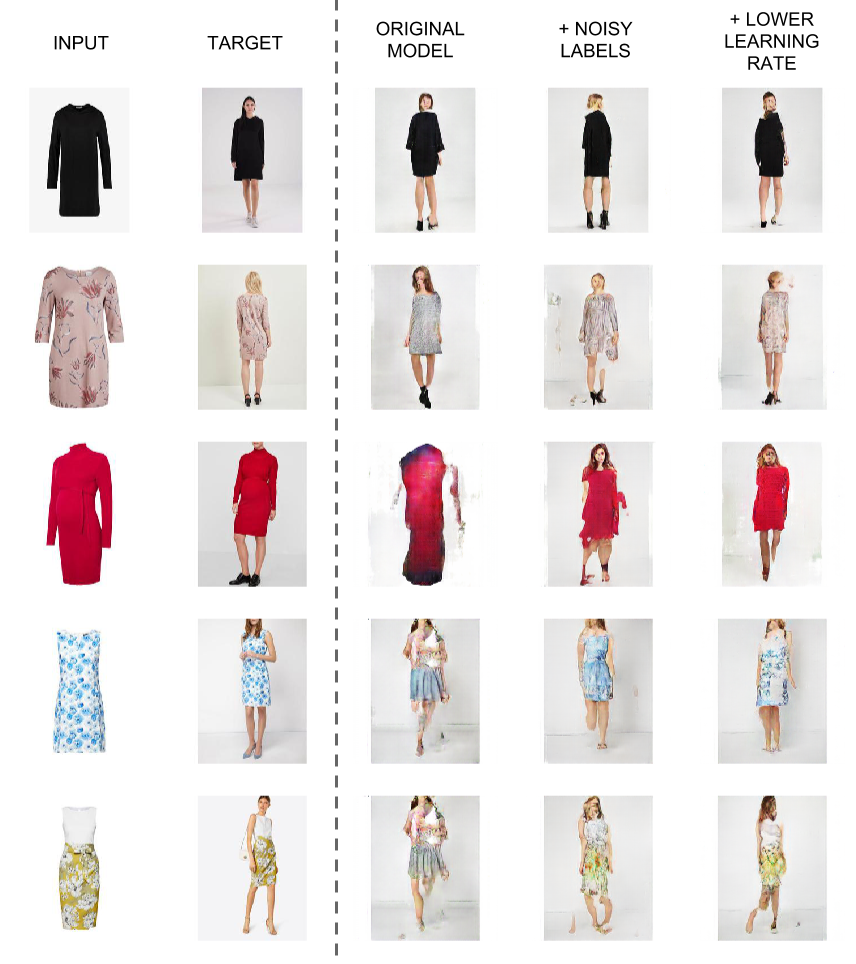
\includegraphics[width=.8\linewidth]{pix2pix/results}}
\caption{\label{fig:pix2pix_results} \textbf{Generated test set images of pix2pix model with different modifications.} The first two columns show the input image that the network receives and the corresponding target image. The outputs come from the original implementation of the model, model with added label noise to confuse the discriminator and a model with learning rate 0.0001 respectively.}
\end{figure}

The original model produces visually inconsistent results: some generated outputs look realistic enough, as product 1 and 2, while others seem to fail. For example, for products 4 and 5, the generator produces almost identical output with a slight change of color.

We can observe that the model which uses noisy labels, where the discriminator is not as strong, does not have these issues and overall produces more stable results. The same model trained with a lower learning rate is better at capturing the textures of the input image. 



% ==============================================================
% PRODUCTS TO MODELS
% ==============================================================
\pagebreak
\subsection{Shape Modification}
The fashion dataset contains multiple attributes that can be modified to allow the user to "tailor" a product according to their taste and trigger a new product search. Aside from color and pattern of the products, the goal is to also modify their shapes - such as change the length of the sleeves or change a V-neck to a round neckline.

This task requires an unsupervised approach, as there are no image pairs of the same product in a sleeveless and a long-sleeved version. Moreover, the task is multi-domain, meaning that the shape attribute is not binary, but has multiple domains, such as short sleeves, long sleeves or sleeveless. 

Based on these requirements, the obvious choice is the StarGAN, for its unsupervised and multi-domain nature. I have used the official StarGAN implementation written in PyTorch to train the models: \hyperlink{https://github.com/sonynka/StarGAN}{github.com/sonynka/StarGAN}.

I have experimented with various shape attributes from the dataset, summarized in Table \ref{tab:shape_attr}. Theoretically, StarGAN should be able to learn one generator mapping for all the attributes and their values. However, to reduce the complexity of the model, I decided to train one generator per reach attribute.

\begin{table}[h]
\centering
\begin{tabular}{*{2}{l}}
Attribute & Possible Values \\
\hline
Sleeve Length			& long, half, short, sleeveless \\
Neckline  				& back, deep, lined, round, v, wide \\
Length					& long, 3/4, knee, normal, short \\
Fit			 			& normal, loose, tight \\
\end{tabular}
\caption{\label{tab:shape_attr}\textbf{Shape attributes of the fashion dataset and their values.} %Supervised training means that the dataset consists of image pairs, e.g: a dress and a person wearing the dress. Multi-Domain networks are able to train one model to change multiple attributes. Multi-Modal networks are able to generate more than one possible output. Networks with latent representations try to model the training data in a latent space, as opposed to pixel space.
}
\end{table}


\begin{figure}[h]
\centering
\subcaptionbox{Discriminator}{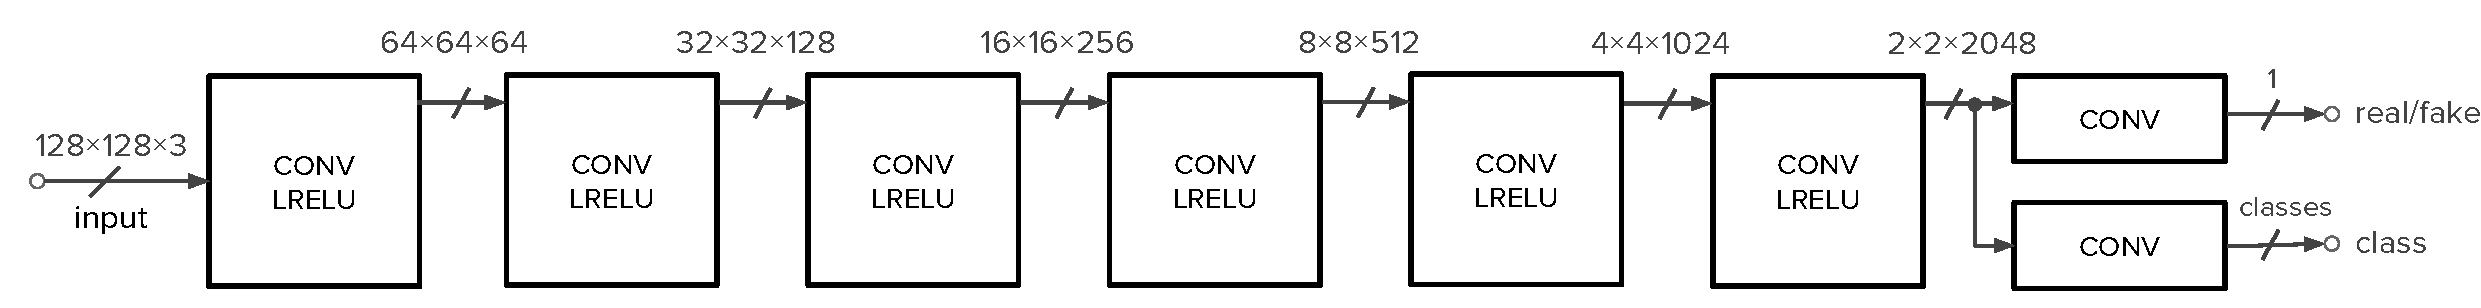
\includegraphics[width=\linewidth]{stargan/dis_arch}}\vspace{.5cm}
\subcaptionbox{Generator}{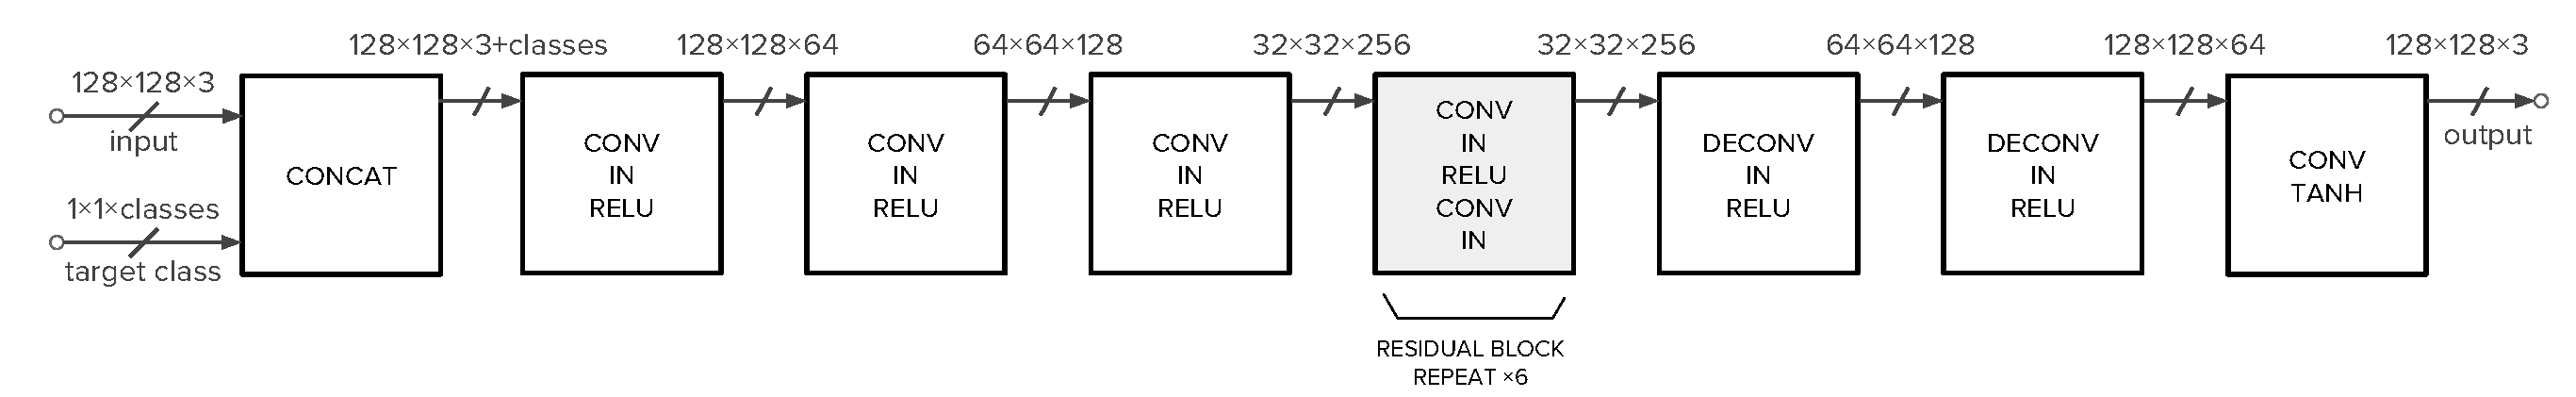
\includegraphics[width=\linewidth]{stargan/gen_arch}}
\caption{\label{fig:stargan_arch} \textbf{Experiment StarGAN Architecture.} The architecture of the trained  discriminator and generator. CONV denotes a convolutional layer, IN denotes instance normalization, LRELU denotes leaky relu with slope 0.2.}
\end{figure}


\paragraph{Sleeve Length}


% ==============================================================
% IMAGE RETRIEVAL
% ==============================================================
\pagebreak
\subsection{Image Retrieval}

\subsubsection{Dataset Images}
In this part of the image features comparison, I have used the original product images from the dataset as input to retrieve the most similar images. All feature distances were calculated using L2 distance. Figure \ref{fig:search_pink} illustrates the strengths and weaknesses of the tested feature vectors. 

Akiwi50 retrieves images that have similar color palettes but different shapes, while Akiwi64 does the opposite: it retrieves similarly shaped products regardless of their color. Although the two features combined together return more sensible results, given that the input dress is not very unique in the dataset, the results are still not very accurate. 

The ResNet features are quite similar, however in both ResNet and ResNet retrained there are outliers of images that do not fit color-wise. The combination of the original ResNet feature with the color-focused Akiwi50 prevents this issue and returns the most similar images. 

\begin{figure}[h]
\centering
{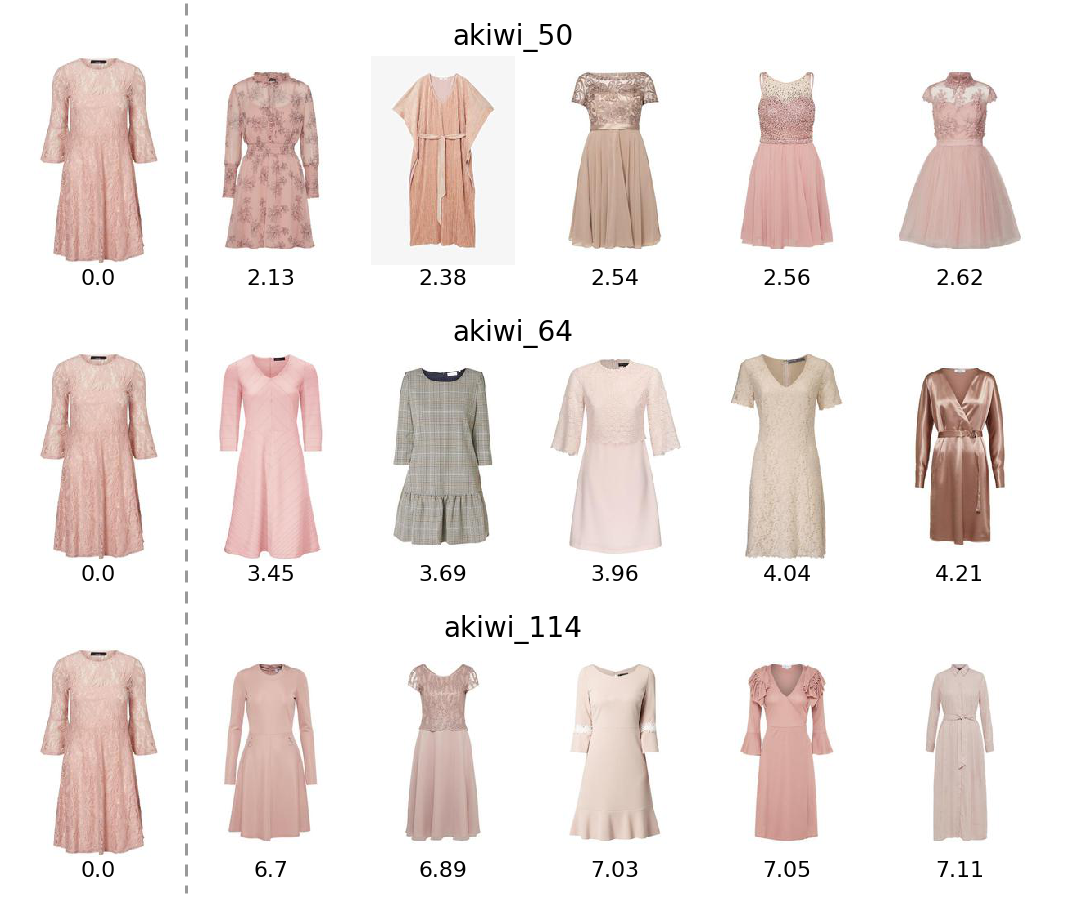
\includegraphics[width=.48\linewidth]{retrieval_exp/akiwi_pink}}\hspace{0.2cm}
{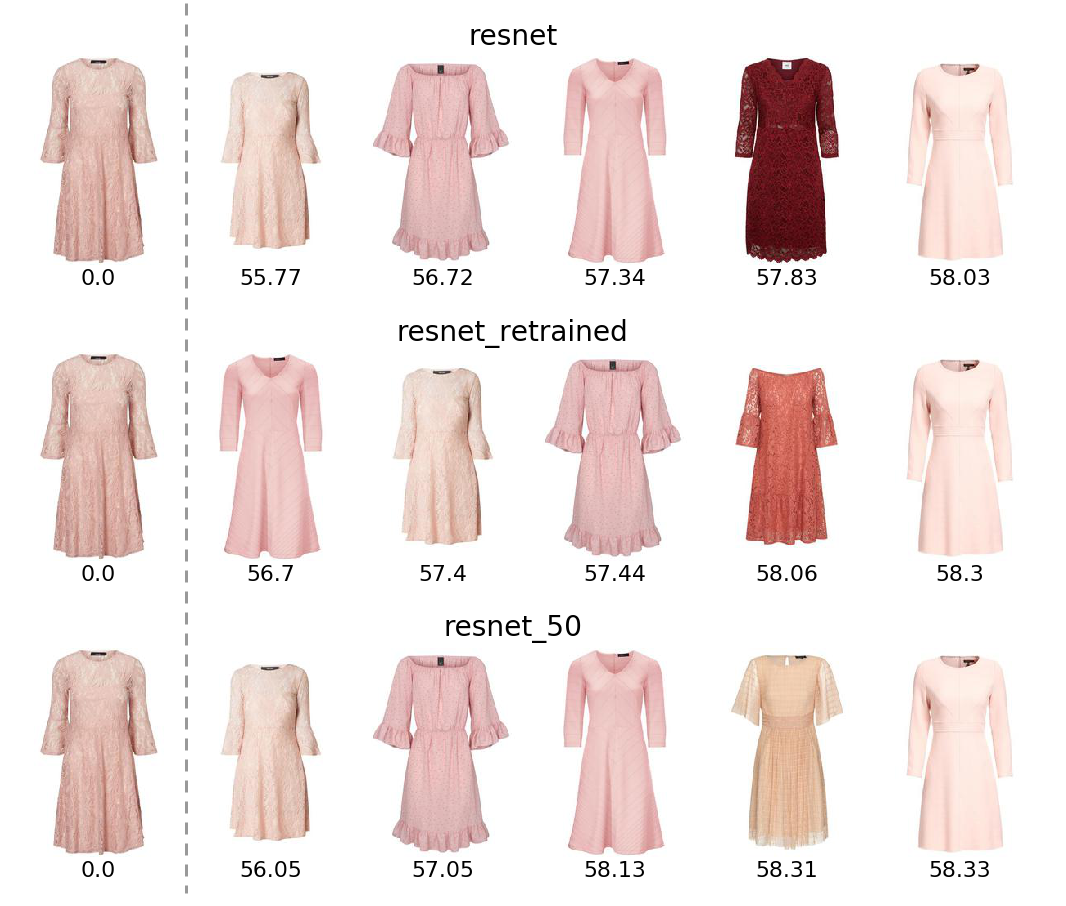
\includegraphics[width=.48\linewidth]{retrieval_exp/resnet_pink}}
\caption{\label{fig:search_pink} \textbf{Image retrieval results with tested feature vectors.} The left shows the Akiwi Features, the right one shows ResNet Features. Each row shows the input image in the left column and the best 5 matches based on L2 distance between the respective feature vectors. The number under each image represents its distance to the input}.
\end{figure}

To further analyse the issue of color outliers within ResNet results, I have also tested different weighing combinations of ResNet and Akiwi50 features. Figure \ref{fig:search_weights} shows the retrieved images for different relative ratios between the two features, such as 1:1, 1:2 and 1:3 for ResNet and Akiwi50 respectively. 

When using ratio 1:1, as shown in first row, the results still include some outliers in terms of colors. However, ratio 1:3 already depends too strong on the Akiwi50 features and the results include images with fitting color but quite different shape. Therefore I have decided to use the ratio 1:2 of ResNet and Akiwi50 features respectively.

\begin{figure}[!h]
\centering
{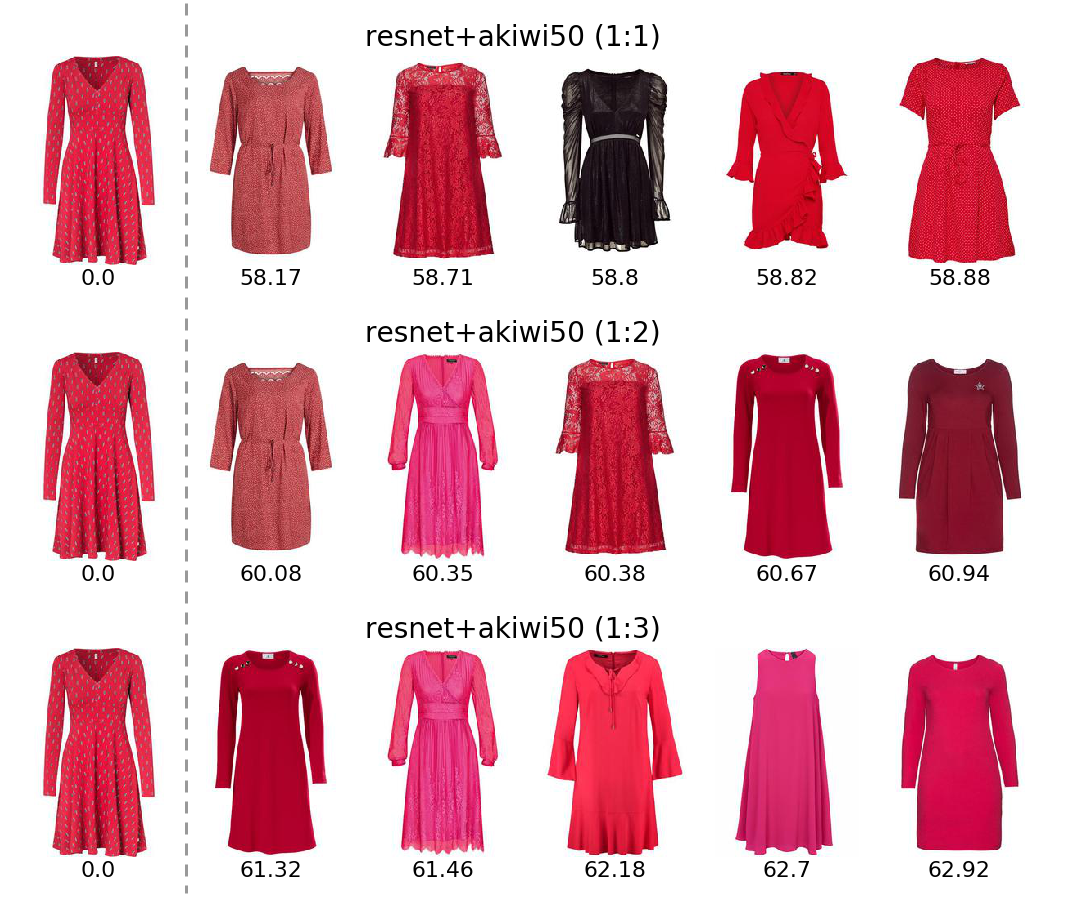
\includegraphics[width=.48\linewidth]{retrieval_exp/resnet_red}}\hspace{0.2cm}
{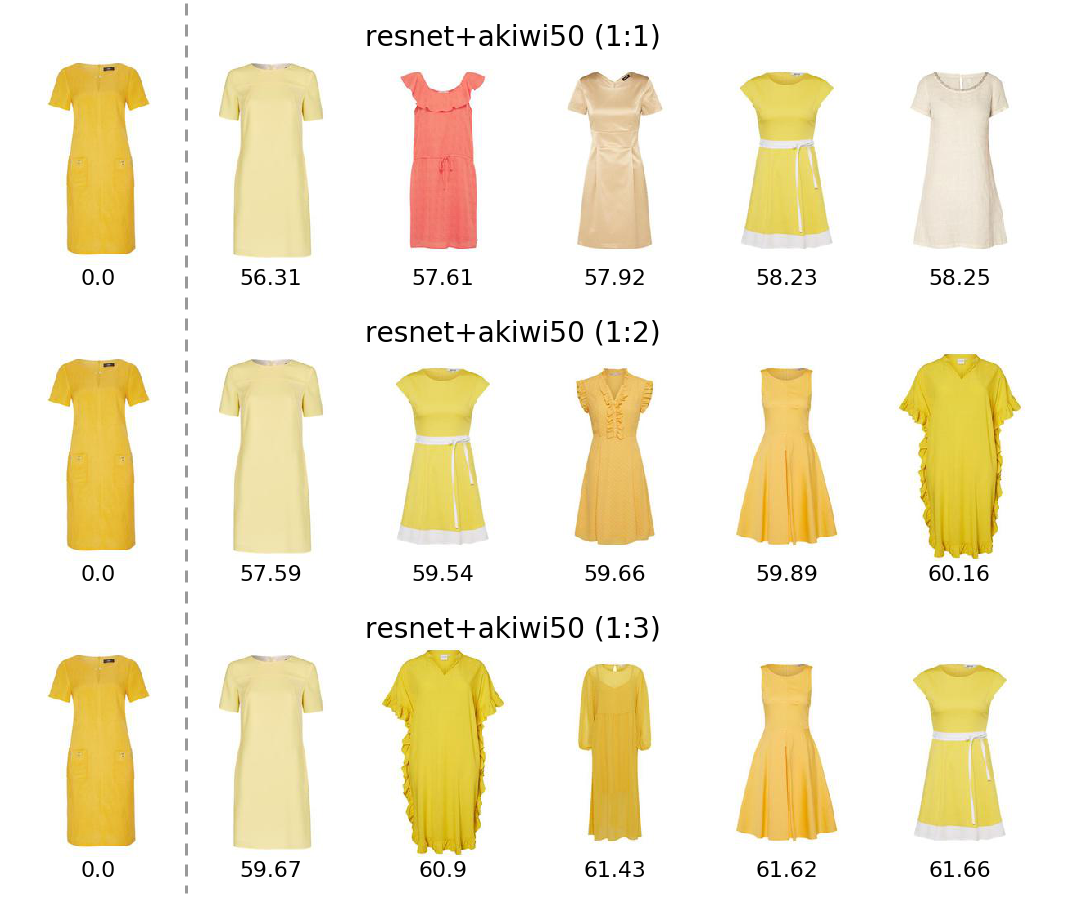
\includegraphics[width=.48\linewidth]{retrieval_exp/resnet_yellow}}
\caption{\label{fig:search_weights} \textbf{Image retrieval results with different combinations of ResNet and Akiwi50 features.} Displaying the results for two different input images, the first row shows an equal ratio, second row shows 1:2 ratio and third row shows 1:3 ratio when combining ResNet and Akiwi50 features respectively.}.
\end{figure}


More examples of results of the image retrieval with different outputs can be found in attachments.

\subsubsection{Generated Images}
















\newpage
\bibliographystyle{abbrvnat}
\bibliography{zotero}
\end{document}
